% The master copy of this demo dissertation is held on my filespace
% on the cl file serve (/homes/mr/teaching/demodissert/)

% Last updated by PMY on 3 March 2012

\documentclass[12pt,twoside,notitlepage,xetex]{report}

\usepackage{a4}
\usepackage{verbatim}
\usepackage{epsf}
\usepackage{sectsty}

\usepackage{url}
\usepackage{parskip}
\usepackage{pdfpages}
% \usepackage{wrapfig}
\usepackage{subfig}
\usepackage[normalem]{ulem}
\usepackage{caption}
\usepackage{color}
\usepackage{float}
% \usepackage{lettrine} % dropped capitals at start of chapter
\usepackage{fancyvrb}
% \usepackage{cprotect}
\usepackage{lscape}

\usepackage{graphicx}
\usepackage{fontspec,xunicode}
\defaultfontfeatures{Mapping=tex-text, Numbers=Monospaced}% ,Scale=MatchLowercase% , Numbers=OldStyle
\setmainfont[Scale=1]{Linux Libertine O}% {Sabon MT Std}
\setsansfont{Roboto Bold}% {Myriad Pro Light}
\setmonofont[Scale=0.82]{Monaco}% {Droid Sans Mono}
\allsectionsfont{\sffamily}

\newfontinstance\bigsf[Color=000000,Scale=1.25]{Roboto Bold}% {Myriad Pro Light}
\newfontinstance\sfapp[Color=000000,Scale=0.82]{Roboto Regular}% {Myriad Pro Light}

\definecolor{red}{rgb}{0.80,0.00,0.00}
\definecolor{green}{rgb}{0.00,0.80,0.00}
\definecolor{blue}{rgb}{0.00,0.00,0.80}

%%% ====================================================================
%%%   This file is freely redistributable and placed into the
%%%   public domain by Tomas Rokicki.
%%%  @TeX-file{
%%%     author          = "Tom Rokicki",
%%%     version         = "2.7k",
%%%     date            = "19 July 1997",
%%%     time            = "10:00:05 MDT",
%%%     filename        = "epsf.tex",
%%%     address         = "Tom Rokicki
%%%                        Box 2081
%%%                        Stanford, CA 94309
%%%                        USA",
%%%     telephone       = "+1 415 855 9989",
%%%     email           = "rokicki@cs.stanford.edu (Internet)",
%%%     codetable       = "ISO/ASCII",
%%%     keywords        = "PostScript, TeX",
%%%     supported       = "yes",
%%%     abstract        = "This file contains macros to support the inclusion
%%%                        of Encapsulated PostScript files in TeX documents.",
%%%     docstring       = "This file contains TeX macros to include an
%%%                        Encapsulated PostScript graphic.  It works
%%%                        by finding the bounding box comment,
%%%                        calculating the correct scale values, and
%%%                        inserting a vbox of the appropriate size at
%%%                        the current position in the TeX document.
%%%
%%%                        To use, simply say
%%%
%%%                        \input epsf % somewhere early on in your TeX file
%%%
%%%                        % then where you want to insert a vbox for a figure:
%%%                        \epsfbox{filename.ps}
%%%
%%%                        Alternatively, you can supply your own
%%%                        bounding box by
%%%
%%%                        \epsfbox[0 0 30 50]{filename.ps}
%%%
%%%                        This will not read in the file, and will
%%%                        instead use the bounding box you specify.
%%%
%%%                        The effect will be to typeset the figure as
%%%                        a TeX box, at the point of your \epsfbox
%%%                        command. By default, the graphic will have
%%%                        its `natural' width (namely the width of
%%%                        its bounding box, as described in
%%%                        filename.ps). The TeX box will have depth
%%%                        zero.
%%%
%%%                        You can enlarge or reduce the figure by
%%%                        saying
%%%
%%%                          \epsfxsize=<dimen> \epsfbox{filename.ps}
%%%                        or
%%%                          \epsfysize=<dimen> \epsfbox{filename.ps}
%%%
%%%                        instead. Then the width of the TeX box will
%%%                        be \epsfxsize and its height will be scaled
%%%                        proportionately (or the height will be
%%%                        \epsfysize and its width will be scaled
%%%                        proportionately).
%%%
%%%                        The width (and height) is restored to zero
%%%                        after each use, so \epsfxsize or \epsfysize
%%%                        must be specified before EACH use of
%%%                        \epsfbox.
%%%
%%%                        A more general facility for sizing is
%%%                        available by defining the \epsfsize macro.
%%%                        Normally you can redefine this macro to do
%%%                        almost anything.  The first parameter is
%%%                        the natural x size of the PostScript
%%%                        graphic, the second parameter is the
%%%                        natural y size of the PostScript graphic.
%%%                        It must return the xsize to use, or 0 if
%%%                        natural scaling is to be used.  Common uses
%%%                        include:
%%%
%%%                           \epsfxsize  % just leave the old value alone
%%%                           0pt         % use the natural sizes
%%%                           #1          % use the natural sizes
%%%                           \hsize      % scale to full width
%%%                           0.5#1       % scale to 50% of natural size
%%%                           \ifnum #1>\hsize\hsize\else#1\fi
%%%                                       % smaller of natural, hsize
%%%
%%%                        If you want TeX to report the size of the
%%%                        figure (as a message on your terminal when
%%%                        it processes each figure), say
%%%                        `\epsfverbosetrue'.
%%%
%%%                        If you only want to get the bounding box
%%%                        extents, without producing any output boxes
%%%                        or \special{}, then say
%%%                        \epsfgetbb{filename}.  The extents will be
%%%                        saved in the macros \epsfllx \epsflly
%%%                        \epsfurx \epsfury in PostScript units of
%%%                        big points.
%%%
%%%                        Revision history:
%%%
%%%                        ---------------------------------------------
%%%                        epsf.tex macro file:
%%%                        Originally written by Tomas Rokicki of
%%%                        Radical Eye Software, 29 Mar 1989.
%%%
%%%                        ---------------------------------------------
%%%                        Revised by Don Knuth, 3 Jan 1990.
%%%
%%%                        ---------------------------------------------
%%%                        Revised by Tomas Rokicki, 18 Jul 1990.
%%%                        Accept bounding boxes with no space after
%%%                        the colon.
%%%
%%%                        ---------------------------------------------
%%%                        Revised by Nelson H. F. Beebe
%%%                        <beebe@math.utah.edu>, 03 Dec 1991 [2.0].
%%%                        Add version number and date typeout.
%%%
%%%                        Use \immediate\write16 instead of \message
%%%                        to ensure output on new line.
%%%
%%%                        Handle nested EPS files.
%%%
%%%                        Handle %%BoundingBox: (atend) lines.
%%%
%%%                        Do not quit when blank lines are found.
%%%
%%%                        Add a few percents to remove generation of
%%%                        spurious blank space.
%%%
%%%                        Move \special output to
%%%                        \epsfspecial{filename} so that other macro
%%%                        packages can input this one, then change
%%%                        the definition of \epsfspecial to match
%%%                        another DVI driver.
%%%
%%%                        Move size computation to \epsfsetsize which
%%%                        can be called by the user; the verbose
%%%                        output of the bounding box and scaled width
%%%                        and height happens here.
%%%
%%%                        ---------------------------------------------
%%%                        Revised by Nelson H. F. Beebe
%%%                        <beebe@math.utah.edu>, 05 May 1992 [2.1].
%%%                        Wrap \leavevmode\hbox{} around \vbox{} with
%%%                        the \special so that \epsffile{} can be
%%%                        used inside \begin{center}...\end{center}
%%%
%%%                        ---------------------------------------------
%%%                        Revised by Nelson H. F. Beebe
%%%                        <beebe@math.utah.edu>, 09 Dec 1992 [2.2].
%%%                        Introduce \epsfshow{true,false} and
%%%                        \epsfframe{true,false} macros; the latter
%%%                        suppresses the insertion of the PostScript,
%%%                        and instead just creates an empty box,
%%%                        which may be handy for rapid prototyping.
%%%
%%%                        ---------------------------------------------
%%%                        Revised by Nelson H. F. Beebe
%%%                        <beebe@math.utah.edu>, 14 Dec 1992 [2.3].
%%%                        Add \epsfshowfilename{true,false}.  When
%%%                        true, and \epsfshowfalse is specified, the
%%%                        PostScript file name will be displayed
%%%                        centered in the figure box.
%%%
%%%                        ---------------------------------------------
%%%                        Revised by Nelson H. F. Beebe
%%%                        <beebe@math.utah.edu>, 20 June 1993 [2.4].
%%%                        Remove non-zero debug setting of \epsfframemargin,
%%%                        and change margin handling to preserve EPS image
%%%                        size and aspect ratio, so that the actual
%%%                        box is \epsfxsize+\epsfframemargin wide by
%%%                        \epsfysize+\epsfframemargin high.
%%%                        Reduce output of \epsfshowfilenametrue to
%%%                        just the bare file name.
%%%
%%%                        ---------------------------------------------
%%%                        Revised by Nelson H. F. Beebe
%%%                        <beebe@math.utah.edu>, 13 July 1993 [2.5].
%%%                        Add \epsfframethickness for control of
%%%                        \epsfframe frame lines.
%%%
%%%                        ---------------------------------------------
%%%                        Revised by Nelson H. F. Beebe
%%%                        <beebe@math.utah.edu>, 02 July 1996 [2.6]
%%%                        Add missing initialization \epsfatendfalse;
%%%                        the lack of this resulted in the wrong
%%%                        BoundingBox being picked up, mea culpa, sigh...
%%%                        ---------------------------------------------
%%%
%%%                        ---------------------------------------------
%%%                        Revised by Nelson H. F. Beebe
%%%                        <beebe@math.utah.edu>, 25 October 1996 [2.7]
%%%                        Update to match changes in from dvips 5-600
%%%                        distribution: new user-accessible macros:
%%%                        \epsfclipon, \epsfclipoff, \epsfdrafton,
%%%                        \epsfdraftoff, change \empty to \epsfempty.
%%%                        ---------------------------------------------
%%%                        
%%%                        Modified to avoid verbosity, give help.
%%%                        --kb@cs.umb.edu, for Texinfo.
%%%  }
%%% ====================================================================
%
\ifx\epsfannounce\undefined \def\epsfannounce{\immediate\write16}\fi
 \epsfannounce{This is `epsf.tex' v2.7k <10 July 1997>}%
%
\newread\epsffilein    % file to \read
\newif\ifepsfatend     % need to scan to LAST %%BoundingBox comment?
\newif\ifepsfbbfound   % success?
\newif\ifepsfdraft     % use draft mode?
\newif\ifepsffileok    % continue looking for the bounding box?
\newif\ifepsfframe     % frame the bounding box?
\newif\ifepsfshow      % show PostScript file, or just bounding box?
\epsfshowtrue          % default is to display PostScript file
\newif\ifepsfshowfilename % show the file name if \epsfshowfalse specified?
\newif\ifepsfverbose   % report what you're making?
\newdimen\epsfframemargin % margin between box and frame
\newdimen\epsfframethickness % thickness of frame rules
\newdimen\epsfrsize    % vertical size before scaling
\newdimen\epsftmp      % register for arithmetic manipulation
\newdimen\epsftsize    % horizontal size before scaling
\newdimen\epsfxsize    % horizontal size after scaling
\newdimen\epsfysize    % vertical size after scaling
\newdimen\pspoints     % conversion factor
%
\pspoints = 1bp        % Adobe points are `big'
\epsfxsize = 0pt       % default value, means `use natural size'
\epsfysize = 0pt       % ditto
\epsfframemargin = 0pt % default value: frame box flush around picture
\epsfframethickness = 0.4pt % TeX's default rule thickness
%
\def\epsfbox#1{\global\def\epsfllx{72}\global\def\epsflly{72}%
   \global\def\epsfurx{540}\global\def\epsfury{720}%
   \def\lbracket{[}\def\testit{#1}\ifx\testit\lbracket
   \let\next=\epsfgetlitbb\else\let\next=\epsfnormal\fi\next{#1}}%
%
% We use \epsfgetlitbb if the user specified an explicit bounding box,
% and \epsfnormal otherwise.  Because \epsfgetbb can be called
% separately to retrieve the bounding box, we move the verbose
% printing the bounding box extents and size on the terminal to
% \epsfstatus.  Therefore, when the user provided the bounding box,
% \epsfgetbb will not be called, so we must call \epsfsetsize and
% \epsfstatus ourselves.
%
\def\epsfgetlitbb#1#2 #3 #4 #5]#6{%
   \epsfgrab #2 #3 #4 #5 .\\%
   \epsfsetsize
   \epsfstatus{#6}%
   \epsfsetgraph{#6}%
}%
%
\def\epsfnormal#1{%
    \epsfgetbb{#1}%
    \epsfsetgraph{#1}%
}%
%
\newhelp\epsfnoopenhelp{The PostScript image file must be findable by
TeX, i.e., somewhere in the TEXINPUTS (or equivalent) path.}%
%
\def\epsfgetbb#1{%
%
%   The first thing we need to do is to open the
%   PostScript file, if possible.
%
    \openin\epsffilein=#1
    \ifeof\epsffilein
        \errhelp = \epsfnoopenhelp
        \errmessage{Could not open file #1, ignoring it}%
    \else                       %process the file
        {%                      %start a group to contain catcode changes
            % Make all special characters, except space, to be of type
            % `other' so we process the file in almost verbatim mode
            % (TeXbook, p. 344).
            \chardef\other=12
            \def\do##1{\catcode`##1=\other}%
            \dospecials
            \catcode`\ =10
            \epsffileoktrue         %true while we are looping
            \epsfatendfalse     %[02-Jul-1996]: add forgotten initialization
            \loop               %reading lines from the EPS file
                \read\epsffilein to \epsffileline
                \ifeof\epsffilein %then no more input
                \epsffileokfalse %so set completion flag
            \else                %otherwise process one line
                \expandafter\epsfaux\epsffileline:. \\%
            \fi
            \ifepsffileok
            \repeat
            \ifepsfbbfound
            \else
                \ifepsfverbose
                    \immediate\write16{No BoundingBox comment found in %
                                    file #1; using defaults}%
                \fi
            \fi
        }%                      %end catcode changes
        \closein\epsffilein
    \fi                         %end of file processing
    \epsfsetsize                %compute size parameters
    \epsfstatus{#1}%
}%
%
% Clipping control:
\def\epsfclipon{\def\epsfclipstring{ clip}}%
\def\epsfclipoff{\def\epsfclipstring{\ifepsfdraft\space clip\fi}}%
\epsfclipoff % default for dvips is OFF
%
% The special that is emitted by \epsfsetgraph comes from this macro.
% It is defined separately to allow easy customization by other
% packages that first \input epsf.tex, then redefine \epsfspecial.
% This macro is invoked in the lower-left corner of a box of the
% width and height determined from the arguments to \epsffile, or
% from the %%BoundingBox in the EPS file itself.
%
% This version is for dvips:
\def\epsfspecial#1{%
     \epsftmp=10\epsfxsize
     \divide\epsftmp\pspoints
     \ifnum\epsfrsize=0\relax
       \special{PSfile=\ifepsfdraft psdraft.ps\else#1\fi\space
                llx=\epsfllx\space
                lly=\epsflly\space
                urx=\epsfurx\space
                ury=\epsfury\space
                rwi=\number\epsftmp
                \epsfclipstring
               }%
     \else
       \epsfrsize=10\epsfysize
       \divide\epsfrsize\pspoints
       \special{PSfile=\ifepsfdraft psdraft.ps\else#1\fi\space
                llx=\epsfllx\space
                lly=\epsflly\space
                urx=\epsfurx\space
                ury=\epsfury\space
                rwi=\number\epsftmp\space
                rhi=\number\epsfrsize
                \epsfclipstring
               }%
     \fi
}%
%
% \epsfframe macro adapted from the TeXbook, exercise 21.3, p. 223, 331.
% but modified to set the box width to the natural width, rather
% than the line width, and to include space for margins and rules
\def\epsfframe#1%
{%
  \leavevmode                   % so we can put this inside
                                % a centered environment
  \setbox0 = \hbox{#1}%
  \dimen0 = \wd0                                % natural width of argument
  \advance \dimen0 by 2\epsfframemargin         % plus width of 2 margins
  \advance \dimen0 by 2\epsfframethickness      % plus width of 2 rule lines
  \vbox
  {%
    \hrule height \epsfframethickness depth 0pt
    \hbox to \dimen0
    {%
      \hss
      \vrule width \epsfframethickness
      \kern \epsfframemargin
      \vbox {\kern \epsfframemargin \box0 \kern \epsfframemargin }%
      \kern \epsfframemargin
      \vrule width \epsfframethickness
      \hss
    }% end hbox
    \hrule height 0pt depth \epsfframethickness
  }% end vbox
}%
%
\def\epsfsetgraph#1%
{%
   %
   % Make the vbox and stick in a \special that the DVI driver can
   % parse.  \vfil and \hfil are used to place the \special origin at
   % the lower-left corner of the vbox.  \epsfspecial can be redefined
   % to produce alternate \special syntaxes.
   %
   \leavevmode
   \hbox{% so we can put this in \begin{center}...\end{center}
     \ifepsfframe\expandafter\epsfframe\fi
     {\vbox to\epsfysize
     {%
        \ifepsfshow
            % output \special{} at lower-left corner of figure box
            \vfil
            \hbox to \epsfxsize{\epsfspecial{#1}\hfil}%
        \else
            \vfil
            \hbox to\epsfxsize{%
               \hss
               \ifepsfshowfilename
               {%
                  \epsfframemargin=3pt % local change of margin
                  \epsfframe{{\tt #1}}%
               }%
               \fi
               \hss
            }%
            \vfil
        \fi
     }%
   }}%
   %
   % Reset \epsfxsize and \epsfysize, as documented above.
   %
   \global\epsfxsize=0pt
   \global\epsfysize=0pt
}%
%
%   Now we have to calculate the scale and offset values to use.
%   First we compute the natural sizes.
%
\def\epsfsetsize
{%
   \epsfrsize=\epsfury\pspoints
   \advance\epsfrsize by-\epsflly\pspoints
   \epsftsize=\epsfurx\pspoints
   \advance\epsftsize by-\epsfllx\pspoints
%
%   If `epsfxsize' is 0, we default to the natural size of the picture.
%   Otherwise we scale the graph to be \epsfxsize wide.
%
   \epsfxsize=\epsfsize{\epsftsize}{\epsfrsize}%
   \ifnum \epsfxsize=0
      \ifnum \epsfysize=0
        \epsfxsize=\epsftsize
        \epsfysize=\epsfrsize
        \epsfrsize=0pt
%
%   We have a sticky problem here:  TeX doesn't do floating point arithmetic!
%   Our goal is to compute y = rx/t. The following loop does this reasonably
%   fast, with an error of at most about 16 sp (about 1/4000 pt).
%
      \else
        \epsftmp=\epsftsize \divide\epsftmp\epsfrsize
        \epsfxsize=\epsfysize \multiply\epsfxsize\epsftmp
        \multiply\epsftmp\epsfrsize \advance\epsftsize-\epsftmp
        \epsftmp=\epsfysize
        \loop \advance\epsftsize\epsftsize \divide\epsftmp 2
        \ifnum \epsftmp>0
           \ifnum \epsftsize<\epsfrsize
           \else
              \advance\epsftsize-\epsfrsize \advance\epsfxsize\epsftmp
           \fi
        \repeat
        \epsfrsize=0pt
      \fi
   \else
     \ifnum \epsfysize=0
       \epsftmp=\epsfrsize \divide\epsftmp\epsftsize
       \epsfysize=\epsfxsize \multiply\epsfysize\epsftmp
       \multiply\epsftmp\epsftsize \advance\epsfrsize-\epsftmp
       \epsftmp=\epsfxsize
       \loop \advance\epsfrsize\epsfrsize \divide\epsftmp 2
       \ifnum \epsftmp>0
          \ifnum \epsfrsize<\epsftsize
          \else
             \advance\epsfrsize-\epsftsize \advance\epsfysize\epsftmp
          \fi
       \repeat
       \epsfrsize=0pt
     \else
       \epsfrsize=\epsfysize
     \fi
   \fi
}%
%
% Issue some status messages if the user requested them
%
\def\epsfstatus#1{% arg = filename
   \ifepsfverbose
     \immediate\write16{#1: BoundingBox:
                  llx = \epsfllx\space lly = \epsflly\space
                  urx = \epsfurx\space ury = \epsfury\space}%
     \immediate\write16{#1: scaled width = \the\epsfxsize\space
                  scaled height = \the\epsfysize}%
   \fi
}%
%
%   We still need to define the tricky \epsfaux macro. This requires
%   a couple of magic constants for comparison purposes.
%
{\catcode`\%=12 \global\let\epsfpercent=%\global\def\epsfbblit{%BoundingBox}}%
\global\def\epsfatend{(atend)}%
%
%   So we're ready to check for `%BoundingBox:' and to grab the
%   values if they are found.
%
%   If we find a line
%
%   %%BoundingBox: (atend)
%
%   then we ignore it, but set a flag to force parsing all of the
%   file, so the last %%BoundingBox parsed will be the one used.  This
%   is necessary, because EPS files can themselves contain other EPS
%   files with their own %%BoundingBox comments.
%
%   If we find a line
%
%   %%BoundingBox: llx lly urx ury
%
%   then we save the 4 values in \epsfllx, \epsflly, \epsfurx, \epsfury.
%   Then, if we have not previously parsed an (atend), we flag completion
%   and can stop reading the file.  Otherwise, we must keep on reading
%   to end of file so that we find the values on the LAST %%BoundingBox.
\long\def\epsfaux#1#2:#3\\%
{%
   \def\testit{#2}%             % save second character up to just before colon
   \ifx#1\epsfpercent           % then first char is percent (quick test)
       \ifx\testit\epsfbblit    % then (slow test) we have %%BoundingBox
            \epsfgrab #3 . . . \\%
            \ifx\epsfllx\epsfatend % then ignore %%BoundingBox: (atend)
                \global\epsfatendtrue
            \else               % else found %%BoundingBox: llx lly urx ury
                \ifepsfatend    % then keep parsing ALL %%BoundingBox lines
                \else           % else stop after first one parsed
                    \epsffileokfalse
                \fi
                \global\epsfbbfoundtrue
            \fi
       \fi
   \fi
}%
%
%   Here we grab the values and stuff them in the appropriate definitions.
%
\def\epsfempty{}%
\def\epsfgrab #1 #2 #3 #4 #5\\{%
   \global\def\epsfllx{#1}\ifx\epsfllx\epsfempty
      \epsfgrab #2 #3 #4 #5 .\\\else
   \global\def\epsflly{#2}%
   \global\def\epsfurx{#3}\global\def\epsfury{#4}\fi
}%
%
%   We default the epsfsize macro.
%
\def\epsfsize#1#2{\epsfxsize}%
%
%   Finally, another definition for compatibility with older macros.
%
\let\epsffile=\epsfbox
\endinput
                            % to allow postscript inclusions
% On thor and CUS read top of file:
%     /opt/TeX/lib/texmf/tex/dvips/epsf.sty
% On CL machines read:
%     /usr/lib/tex/macros/dvips/epsf.tex

\raggedbottom                           % try to avoid widows and orphans
\raggedright                            % left-aligned, not justified
\sloppy
\clubpenalty1000%
\widowpenalty1000%

\addtolength{\oddsidemargin}{6mm}       % adjust margins
\addtolength{\evensidemargin}{-8mm}

\renewcommand{\baselinestretch}{1.1}    % adjust line spacing to make
                                        % more readable

\renewcommand{\captionfont}{\footnotesize}

\setcounter{secnumdepth}{5}
% \setcounter{tocdepth}{5}

\begin{document}
\nocite{*}
\bibliographystyle{plain}% {unsrt}


%%%%%%%%%%%%%%%%%%%%%%%%%%%%%%%%%%%%%%%%%%%%%%%%%%%%%%%%%%%%%%%%%%%%%%%%
% Title


\pagestyle{empty}

% \hfill{\LARGE \bf \sffamily Philip Yeeles}
\hfill{\Large Philip Yeeles}

\vspace*{60mm}
\begin{center}
\LARGE
{\bf \bigsf Nico: An Environment for Mathematical Expression in Schools}\\
\vspace*{5mm}
% {\sffamily Computer Science Tripos} \\
Computer Science Tripos\\
\vspace*{5mm}
% {\sffamily Selwyn College} \\
Selwyn College\\
\vspace*{5mm}
% {\sffamily \today}  % today's date
\today % today's date
\end{center}

\cleardoublepage

%%%%%%%%%%%%%%%%%%%%%%%%%%%%%%%%%%%%%%%%%%%%%%%%%%%%%%%%%%%%%%%%%%%%%%%%%%%%%%
% Proforma, table of contents and list of figures

\setcounter{page}{1}
\pagenumbering{roman}
\pagestyle{plain}

\chapter*{Proforma}

{\large
\begin{tabular}{ll}
\bf Name:               & Philip Yeeles                                                   \\
\bf College:            & Selwyn College                                                  \\
\bf Project Title:      & Nico: An Environment for Mathematical\\
                        & Expression in Schools \\
\bf Examination:        & Computer Science Tripos, May 2012                               \\
\bf Word Count:         & TBC\footnotemark[1]
(well less than the 12000 limit) \\
\bf Project Originator: & P.~M.~Yeeles (\verb¬pmy22¬)                                    \\
\bf Supervisors:        & Dr S.~J.~Aaron (\verb¬sja55¬), A.~G.~Stead (\verb¬ags46¬)     \\
\end{tabular}
}
\footnotetext[1]{This word count was computed
by {\tt detex diss.tex | tr -cd '0-9A-Za-z $\tt\backslash$n' | wc -w}
}
\stepcounter{footnote}


\section*{Original Aims of the Project}

The aim of the project was to develop an application in the Clojure programming
language which would allow users to express mathematical calculations using a
graphical notation.  The software was to be able to generate an abstract syntax
tree from the graphical notation, evaluate it and pass the results back to the
application in under 300ms.  An extension to the project was to conduct a user
study to evaluate the utility of the software.
%
% To write a demonstration dissertation\footnote{A normal footnote without the
% complication of being in a table.} using \LaTeX\ to save
% student's time when writing their own dissertations. The dissertation
% should illustrate how to use the more common \LaTeX\ constructs. It
% should include pictures and diagrams to show how these can be
% incorporated into the dissertation.  It should contain the entire
% \LaTeX\ source of the dissertation and the Makefile.  It should
% explain how to construct an MSDOS disk of the dissertation in
% Postscript format that can be used by the book shop for printing, and,
% finally, it should have the prescribed layout and format of a diploma
% dissertation.


\section*{Work Completed}

I have successfully designed and implemented the application detailed in the
previous section.  That is, I have developed an application in which it is
possible to express calculations using a graphical notation, that generates an
abstract syntax tree from the language and that is able to parse the tree and
return the results in under 300ms.  I have also conducted a user study to assess
whether or not the software is actually of use with regard to mathematics
education.
%
% All that has been completed appears in this dissertation.

\section*{Special Difficulties}

Learning the Clojure programming language.
%
% Learning how to incorporate encapulated postscript into a \LaTeX\
% document on both CUS and Thor.

\newpage
\section*{Declaration of Originality}

I, Philip Michael Yeeles of Selwyn College, being a candidate for Part
II of the Computer Science Tripos, hereby declare that this dissertation
and the work described in it are my own work, unaided except as may be
specified below, and that the dissertation does not contain material
that has already been used to any substantial extent for a comparable
purpose.

\bigskip
\leftline{Signed}

\medskip
\leftline{Date \today}

\cleardoublepage

\tableofcontents

\listoffigures

\newpage
\section*{Acknowledgements}
My thanks to Luke Church for his advice regarding user studies, and to Alistair
Stead and Sam Aaron for their encouragement and patience.
%
% This document owes much to an earlier version written by Simon Moore
% \cite{Moore95}.  His help, encouragement and advice was greatly
% appreciated.

%%%%%%%%%%%%%%%%%%%%%%%%%%%%%%%%%%%%%%%%%%%%%%%%%%%%%%%%%%%%%%%%%%%%%%%
% now for the chapters

\cleardoublepage        % just to make sure before the page numbering
                        % is changed

\setcounter{page}{1}
\pagenumbering{arabic}
\pagestyle{headings}

\chapter{Introduction}
% TODO: sort out cogdims: apparently the proper way to do it is to mention cogdims and cite petra & green, then put all the cogdims terms in italics

% \lettrine{T}{he}
The aim of this project has been to design and develop a notation and
accompanying application to act as a learning aid for pre-algebra arithmetic by
increasing visibility, reducing the number of hidden dependencies and making the
flow of data obvious to the user.  I have successfully developed such a system,
intended initially for pupils in Year 5 (though extensible, through the creation
of alternative question sets, to other age groups), and, as an extension,
conducted a user study to assess its utility.

In this chapter, I will discuss my motivations for choosing this project, the
pros and cons of the handwritten system it is attempting to augment, the
technical challenges involved in developing such a system and related work that
has previously been conducted with similar goals.

\section{Motivations}
% evaluation of problems with writing it down on paper
% cogdims of handwritten method(s)
% system requirements (cogdims)

My motivations behind this project lay in the limitations of the handwritten
approach to solving mathematical problems that I had observed both in my own
learning and in my own teaching experience.  What follows is an evaluation of
the pros and cons of the handwritten method of performing arithmetic
calculations according to Blackwell and Green's ``Cognitive Dimensions''
framework \cite{Blackwell1998}, and a discussion of the properties a useful
alternative notation should have.

\pagebreak

% \subsection{Evaluation of the Handwritten Approach}
% % moved to chapter 2 requirements analysis

% \subsection{Requirements of a Replacement System}
% % moved to chapter 2 requirements analysis

\section{Technical Challenges}
% need first-class functions
% need to be able to pass expressions around to evaluate at will: hence functional, hence lisp - homoiconicity
% also need good gui libraries for app - familiar with java/swing so that works (esp. with seesaw), also the option of jfx2 and swt/guiftw
% difficulty of learning clojure over summer in preparation

Developing such an application comprises two main challenges: developing a
back-end that is capable of creating, storing, editing, deleting, evaluating,
nesting and calculations, and a graphical, user-facing frontend that is able to
render calculations into the devised notation, and allow the user to perform
operations upon the notation that affect the underlying calculation.

I chose to use the Clojure language as it provided many features that would
prove to be useful over the course of the application's development.  As a
dialect of LISP, Clojure is a homoiconic programming language -- that is, a
programming language in which code is represented as a data structure -- which
made passing around and performing operations upon calculations themselves,
rather than just their results, considerably easier.  A calculation can simply
be represented as a piece of code, which can then be utilised as needed.

As the user experience is so crucial to the success of the application, it was
also important that there be well-established GUI libraries available.  Clojure
runs on the Java Virtual Machine (JVM), which puts Java's considerable standard
library at one's disposal, whilst still being able to program in a LISP.  As I
am familiar with Java and the Swing GUI libraries, it was advantageous to be
able to leverage this knowledge in designing the application's interface.  In
addition to this, Java's portability was an advantage, due to the wide range of
platforms available both in educational and home settings.  A Java-based
solution standardises the \emph{Nico} experience across many environments.

\section{Previous Work}
% scrubbing calculator http://worrydream.com/ScrubbingCalculator/
% soulver http://www.acqualia.com/soulver/
% neither really targeted at education
% cool stuff at http://worrydream.com/KillMath/ though
% maybe refer to this? http://betterexplained.com/articles/rethinking-arithmetic-a-visual-guide/
% also, this: http://www.ralph-abraham.org/articles/Blurbs/blurb126.shtml
% also, check out espresso and education city stuff, log in to fronter via st. mary's site, uname jyeele1.314, pword b3ach7
% plenty of work been done in making computer maths like paper maths, but not so much the reverse, case in point: http://www.macresearch.org/showcase-review-pi-cubed-iphone-ipod-touch
% also a lot of crap maths games that are essentially a series of qs in disguise, see http://www.time4learning.com/curriculum/try_demos.html
% nico is unabashedly *not* a game, rather a tool, much like a pen or calculator
% problem with calculators?

There already exists a wide variety of educational software for mathematics, but
much of this is in the form of ``games'', in which a series of mathematical
problems to be solved is poorly disguised as a game -- indeed, such problems
would be more accurately said to be embedded into a game, rather than becoming
the game themselves.  Thus, the object becomes not to solve the problems, but to
play the game that happens to surround the problems.  Such software also does
not often offer any means of solving the problems, other than the traditional
pen-and-paper method (with a piece of paper next to the computer screen), or
the mental approach.  Hence, what the user is then presented with is essentially
a game and a worksheet, awkwardly interleaved.  In some cases, it is even
possible for the user to simply press arbitrary buttons until they pass the
questions, effectively removing the maths element of the game and replacing it
with a series of short breaks in gameplay. % citations!

There also exist a few applications intended to represent calculations on a
computer in novel ways.  A relatively common approach to this has been to try
to make on-screen calculations more like on-paper calculations.  \emph{Pi Cubed}
takes this approach by trying to make complex calculations appear as they would
be written in an exam or exercise book \cite{PiCubed}.  \emph{Soulver},
conversely, tries to achieve this by simulating ``back-of-the-envelope''
calculations, whereby notes in English augment the calculation \cite{Soulver}.
Another approach is that of the \emph{Scrubbing Calculator} \cite{ScrubCalc},
which extends the \emph{Soulver}-style environment by helping the user to solve
equations by dragging values to increase and decrease them, showing how changing
a value affects the overall result.  Values can be linked by dragging a line
between them, which means that they are two instances of the same value -- hence
dragging one changes the value at every location in which it appears.  This is a
neat means of visualising equations, but it, too, is not intended for use in
education, and still requires the user to be able to formulate some kind of
equation.  The \emph{Scrubbing Calculator} is more a tool for facilitating
algebraic understanding, as opposed to arithmetic understanding; indeed, it is
inherently a {\bf calculator}, and so does not encourage thinking about how to
work out the arithmetic parts of a calculation manually.

\section{Summary}
% need a system that incorporates these features: foo, bar, baz, quux

Existing educational ``games'' for mathematics either have too much focus on
being a game, rather than helping to learn mathematics, or are such that the
mathematical element is circumventable.  There exists software to aid in
calculation and arithmetic by representing it clearly, but it is not intended
for educational use, and often its purpose is to make on-screen calculations
appear as one would handwrite them.

There is a niche for a tool for use in education that represents calculations in
a visual manner, with a particular focus on making the method by which arithmetic
problems are solved clear.  My project aims to provide an environment in which
the user can explore the many ways in which a problem can be solved using a
novel graphical notation.

\cleardoublepage



\chapter{Preparation}

% In this chapter I will discuss the work that was done prior to beginning the
% project proper.  This includes learning the Clojure programming language and
% researching and auditioning graphical metaphors for calculation.  This chapter
% comprises a requirements analysis, followed by an overview of the system
% architecture and a discussion of the additional tools used in the development of
% the project.
This chapter concerns the work that was completed prior to beginning the
project proper.  It comprises a requirements analysis, followed by a discussion
of the prototyping process of the graphical notation to be implemented in the
final application.  Finally, there will be a brief examination of the tools
used in the development of the project.

\section{Requirements Analysis}
% http://www.cs.fsu.edu/~lacher/courses/COP3331/rad.html
% http://www.nd.gov/itd/files/services/pm/requirements-analysis-guidebook.pdf

% TODO: write about the requirements analysis and why we're doing one

\subsection{Current System}
% move evaluation of handwritten arithmetic from chapter 1 here?

\begin{figure}
% \begin{wrapfigure}{r}{0.5\textwidth}
\begin{center}
\subfloat[]{
\parbox{2cm}{
\begin{center}
{\small
24+35=59\\
12+48=60\\
59+72=131\\
1+60=61\\
131+61=192}
\end{center}}}
\subfloat[]{
\parbox{2cm}{
\begin{center}
{\small
24+35={\color{green}59}\\
12+48={\color{blue}60}\\
{\color{green}59}+72={\color{green}131}\\
1+{\color{blue}60}={\color{blue}61}\\
{\color{green}131}+{\color{blue}61}=192}
\end{center}}}
\subfloat[]{
\parbox{4cm}{
\begin{center}
{\small
24+35= {\color{red}\sout{59}} {\color{green}49}\\
12+48={\color{blue}60}\\
{\color{red}\sout{59}} {\color{green}49}+72= {\color{red}\sout{131}} {\color{green}121}\\
1+{\color{blue}60}={\color{blue}61}\\
{\color{red}\sout{131}} {\color{green}121}+{\color{blue}61}= {\color{red}\sout{192}} 182}
\end{center}}}
\end{center}
\caption{Illustrating the hidden dependencies and viscosity inherent in pre-algebra, handwritten arithmetic.  The original calculation is shown in (a), has its otherwise-hidden dependencies highlighted in (b), and is altered slightly in (c).}
% \end{wrapfigure}
\end{figure}
% cogdims
% taught method without being taught *why* it works
% high viscosity - have to cross things out or start again
% high repetition viscosity
% low knock-on viscosity
% viscosity is acceptable in transcription and incrementation, but harmful to modification and exploration
% hidden dependencies -
% premature commitment - made worse by high repetition viscosity; have to start again if a mistake is made
% premature commitment is certainly very high for traditional calculators
% algebra is abstraction-hungry, arthimetic is abstraction-hating, though can use secondary notation to construct abstractions
% no abstraction barrier to arithmetic though
% secondary notation - notes around calculations
% visibility - visible, but only juxtaposable if juxtaposed at the start (premature commitment) or with the help of secondary notation
There are a number of problems with handwritten, pre-algebra arithmetic that
this project seeks to rectify.  First of all, the fact that it is handwritten
entails a high level of viscosity: it is difficult to make changes to a written
calculation without sacrificing clarity.  In particular, there is a lot of
repetition viscosity involved in the modification of an existing piece of work;
if a number is changed that is used in several calculations, then it is
time-consuming to change it everywhere it appears in the working.  If several
calculations are dependent upon each other, then this entails a lot of knock-on
viscosity in recalculating each stage after changing the number.  This is
exacerbated by the hidden dependencies between chained calculations in
handwritten arithmetic (\emph{Fig. 2.1}).  The problem of hidden dependencies
is made worse by the low juxtaposability of the system; although the notation
is quite visible, in that every calculation can be seen easily on the page,
juxtaposing two sets of calculations entails considerable premature commitment
on the part of the user, as components cannot easily be edited or relocated due
to the system's high viscosity.  Whilst viscosity can be acceptable in some
situations, it is harmful with regard to modification and exploration within a
notational system, once again requiring a non-trivial amount of premature
commitment on the part of the user.  In many cases, it can actually quicker for
the user to start all over again, as opposed to making the changes required to
rectify their calculations.

Handwritten arithmetic does have one key advantage: it has a very low initial
abstraction barrier.  Other than learning the appropriate symbols for each
operation and digit, and how to combine them, the traditional system of
arithmetic allows a learner to begin using it almost immediately.  Algebra, on
the other hand, has a much higher abstraction barrier, requiring the much more
abstract concept of a variable, rather than a set quantity, to be used
effectively.  Although it is possible to add abstractions to arithmetic by the
use of secondary notation, there is no provision for abstraction included in
the primary notation.  It can, therefore, be said that algebra is an
\emph{abstraction-hungry} system, whereas arithmetic is an
\emph{abstraction-hating} system.  Without abstractions, arithmetic is easy to
get started with, but can be a very verbose and inefficient notation with low
visibility, as outlined above.

\subsection{Proposed System}

\subsubsection{Overview}
% cogdims!!
% need to develop useful notation - early studies, talk about other notations we came up with, notations looked at with alistair (get link)
% hidden dependencies - nico shows a data flow representation (p19, blackwell1998) to make dependencies explicit

% TODO: this bit.  not even sure if it should be in the intro...

To improve upon the standard approach of listing the steps comprising a
calculation, a system must acknowledge and try to overcome the drawbacks listed
above.  To this end, I have designed and developed a notational system and
accompanying applciation that aims to overcome many of the disadvantages
inherent in traditional, handwritten arithmetic.  The intention of the system
is to reduce viscosity, increase visibility and to remove many of the hidden
dependencies that beleaguer the traditional method. % TODO: not ahppy with this; not sure it counts as an overview


\subsubsection{Functional Requirements}

To be an improvement upon the current system detailed above, the new system must
satisfy the following properties:-- % TODO: not happy with this
\begin{itemize}
\item Allows the user to create graphical structures representative of complex calculations
\item Provides the user with a suitable environment in which to do so
\item Allows the user to reposition elements of the structure at will
\item Displays the user's current progress
\item Is able to evaluate the correctness of the user's answer
\item Accepts a file containing a set of questions to be answered
\item Displays the current question being answered
\item Progresses through the current question set as the user answers each question correctly
\end{itemize}

\subsubsection{Non-Functional Requirements}

The system must also satisfy a number of requirements outside of its basic
functionality.  These are listed below.
\begin{itemize}
\item Offers a significant improvement in visibility over handwritten arithmetic
\item Offers a significant improvement in juxtaposability over handwritten arithmetic
\item Reduces premature commitment relative to handwritten arithmetic
\item Reduces hidden dependencies relative to handwritten arithmetic
\item Is interactive: is able to pass results back to the user in less than 300ms\footnote{Roca and Rousseau \cite{Roca2004} have this to say on the subject of interactivity: ``An abundance of studies into user tolerance of round-trip latency [...] has been conducted and generally agrees upon the following levels of tolerance: excellent, 0-300ms; good, 300-600ms; poor, 600-700ms; and quality becomes unacceptable [...] in excess of 700ms.''}
\item Is appealing to the target audience of 9- to 10-year-olds without being childish -- must be applicable to a wider audience if needed (e.g. could it be extended for use in adult education?)
\end{itemize}
% talk about needing to be appealing, etc.?
% more details in notes on user interface subsection in chapter 3

% \subsubsection{Use Case}
%
% % diagram?  see wikipedia "use case"
% lol

% \section{System Overview}
% % do we need if in req. analysis?
%
% lol

\section{User Interface}
% section rather than subsection?  def. section if we don't have system overview
% prototypes!  dig out the preliminary drawings, take screenshots of old versions for later

As this project is primarily concerned with human-computer interaction, the
user interface and experience, and the design thereof, constitutes a
significant part of this project.  As such, this section outlines the initial
development stages of the user interface, first introducing several designs for
the graphical notation, and then discussing in more detail three that were
developed further.

\subsection{Prototyping}

\subsubsection{Low-Fidelity Prototyping}

% drawings 'n' shit
% talk about how decided to come up with 20 different designs then thin them out
To try to get some initial ideas for what could become the calculation metaphor
of choice for the project, a target was set of devising at least twenty,
significantly different, potential designs.  These were recorded as very rough
sketches, a few of which were refined in larger examples, and three of which
were deemed good enough to warrant an application mockup, as detailed in
\emph{Sec. 2.2.1.2}.

% \newpage

% \paragraph{Flowgraphs}\hfill

\begin{center}
\begin{figure}[H]
% \begin{wrapfigure}{r}{0.5\textwidth}
\begin{center}
\subfloat[]{
\parbox{4cm}{
\begin{center}
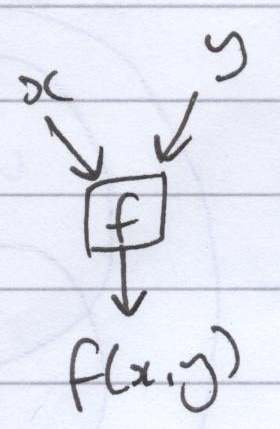
\includegraphics[width=4cm]{figs/mockups/sketches/11/11a.jpg}
\end{center}}}
\subfloat[]{
\parbox{4cm}{
\begin{center}
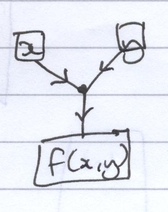
\includegraphics[width=4cm]{figs/mockups/sketches/11/11b.jpg}
\end{center}}}
\end{center}
\caption{Early designs for flowgraph-based calculation metaphors.}
% \end{wrapfigure}
\end{figure}
\end{center}

\begin{center}
\begin{figure}[H]
\begin{center}
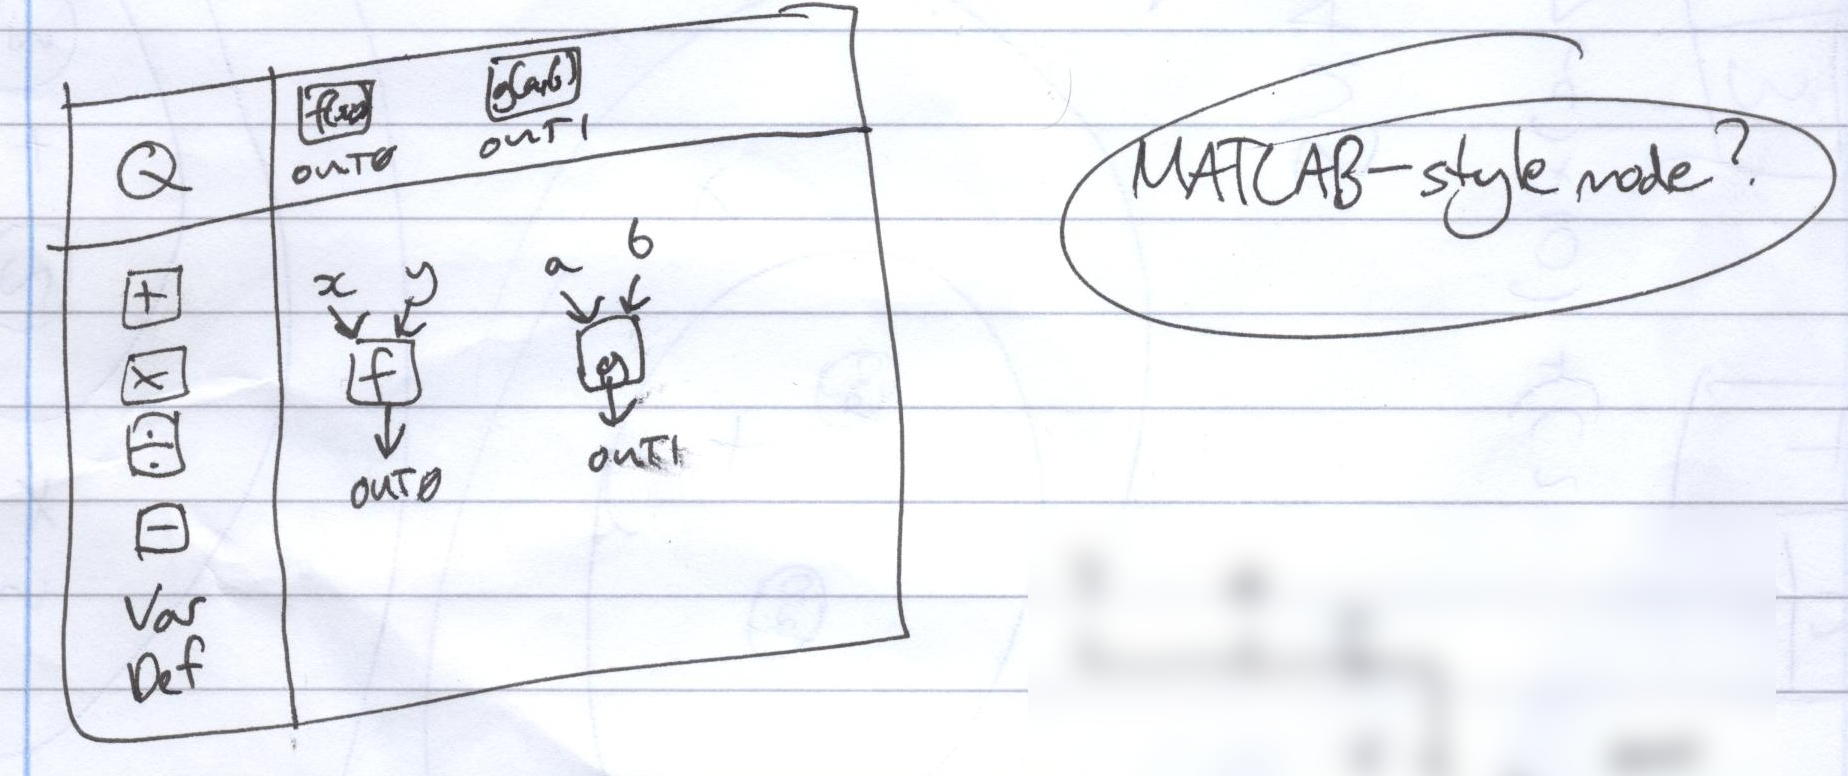
\includegraphics[width=\textwidth]{figs/mockups/sketches/11/11jii.jpg}
\end{center}
\caption{A more refined sketch of a flowgraph-based language and application.}
\end{figure}
\end{center}

% \newpage

% \paragraph{Triangles}\hfill

\begin{center}
\begin{figure}[H]
% \begin{wrapfigure}{r}{0.5\textwidth}
\begin{center}
\subfloat[]{
\parbox{4cm}{
\begin{center}
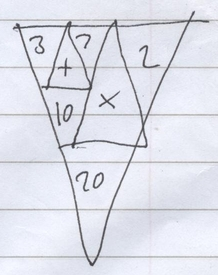
\includegraphics[width=4cm]{figs/mockups/sketches/21/21b.jpg}
\end{center}}}
\subfloat[]{
\parbox{4cm}{
\begin{center}
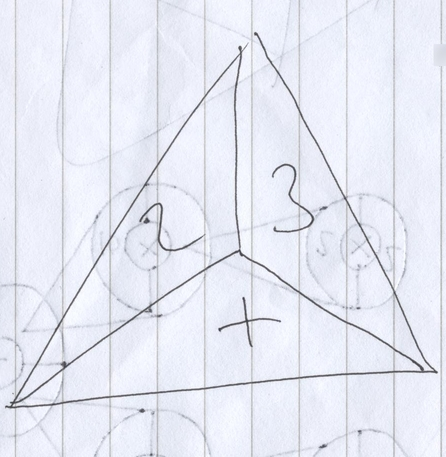
\includegraphics[width=4cm]{figs/mockups/sketches/22/22a.jpg}
\end{center}}}
\subfloat[]{
\parbox{4cm}{
\begin{center}
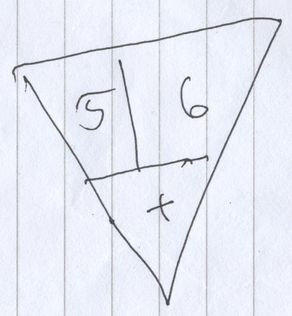
\includegraphics[width=4cm]{figs/mockups/sketches/22/22b.jpg}
\end{center}}}\\
\subfloat[]{
\parbox{4cm}{
\begin{center}
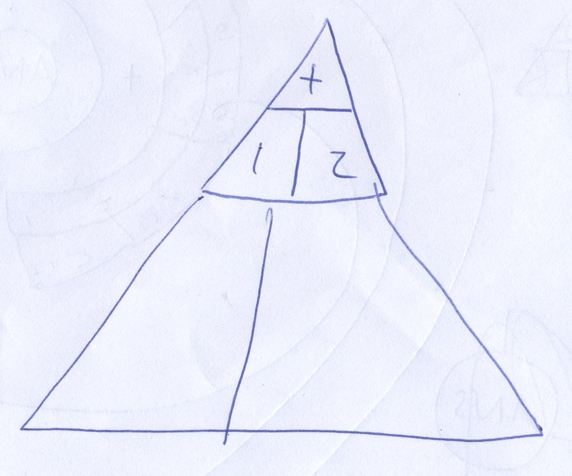
\includegraphics[width=4cm]{figs/mockups/sketches/42/42a.jpg}
\end{center}}}
\subfloat[]{
\parbox{4cm}{
\begin{center}
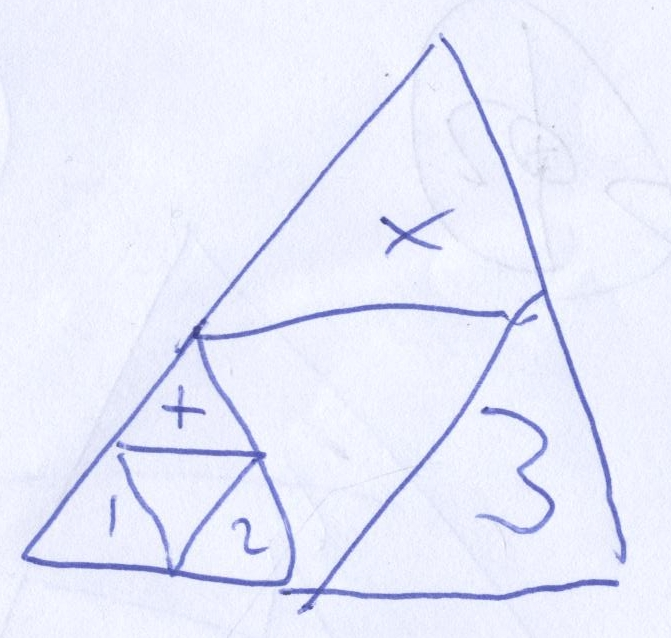
\includegraphics[width=4cm]{figs/mockups/sketches/42/42b.jpg}
\end{center}}}
\end{center}
\caption{Early designs for triangle-based calculation metaphors.}
% \end{wrapfigure}
\end{figure}
\end{center}

\begin{center}
\begin{figure}
\begin{center}
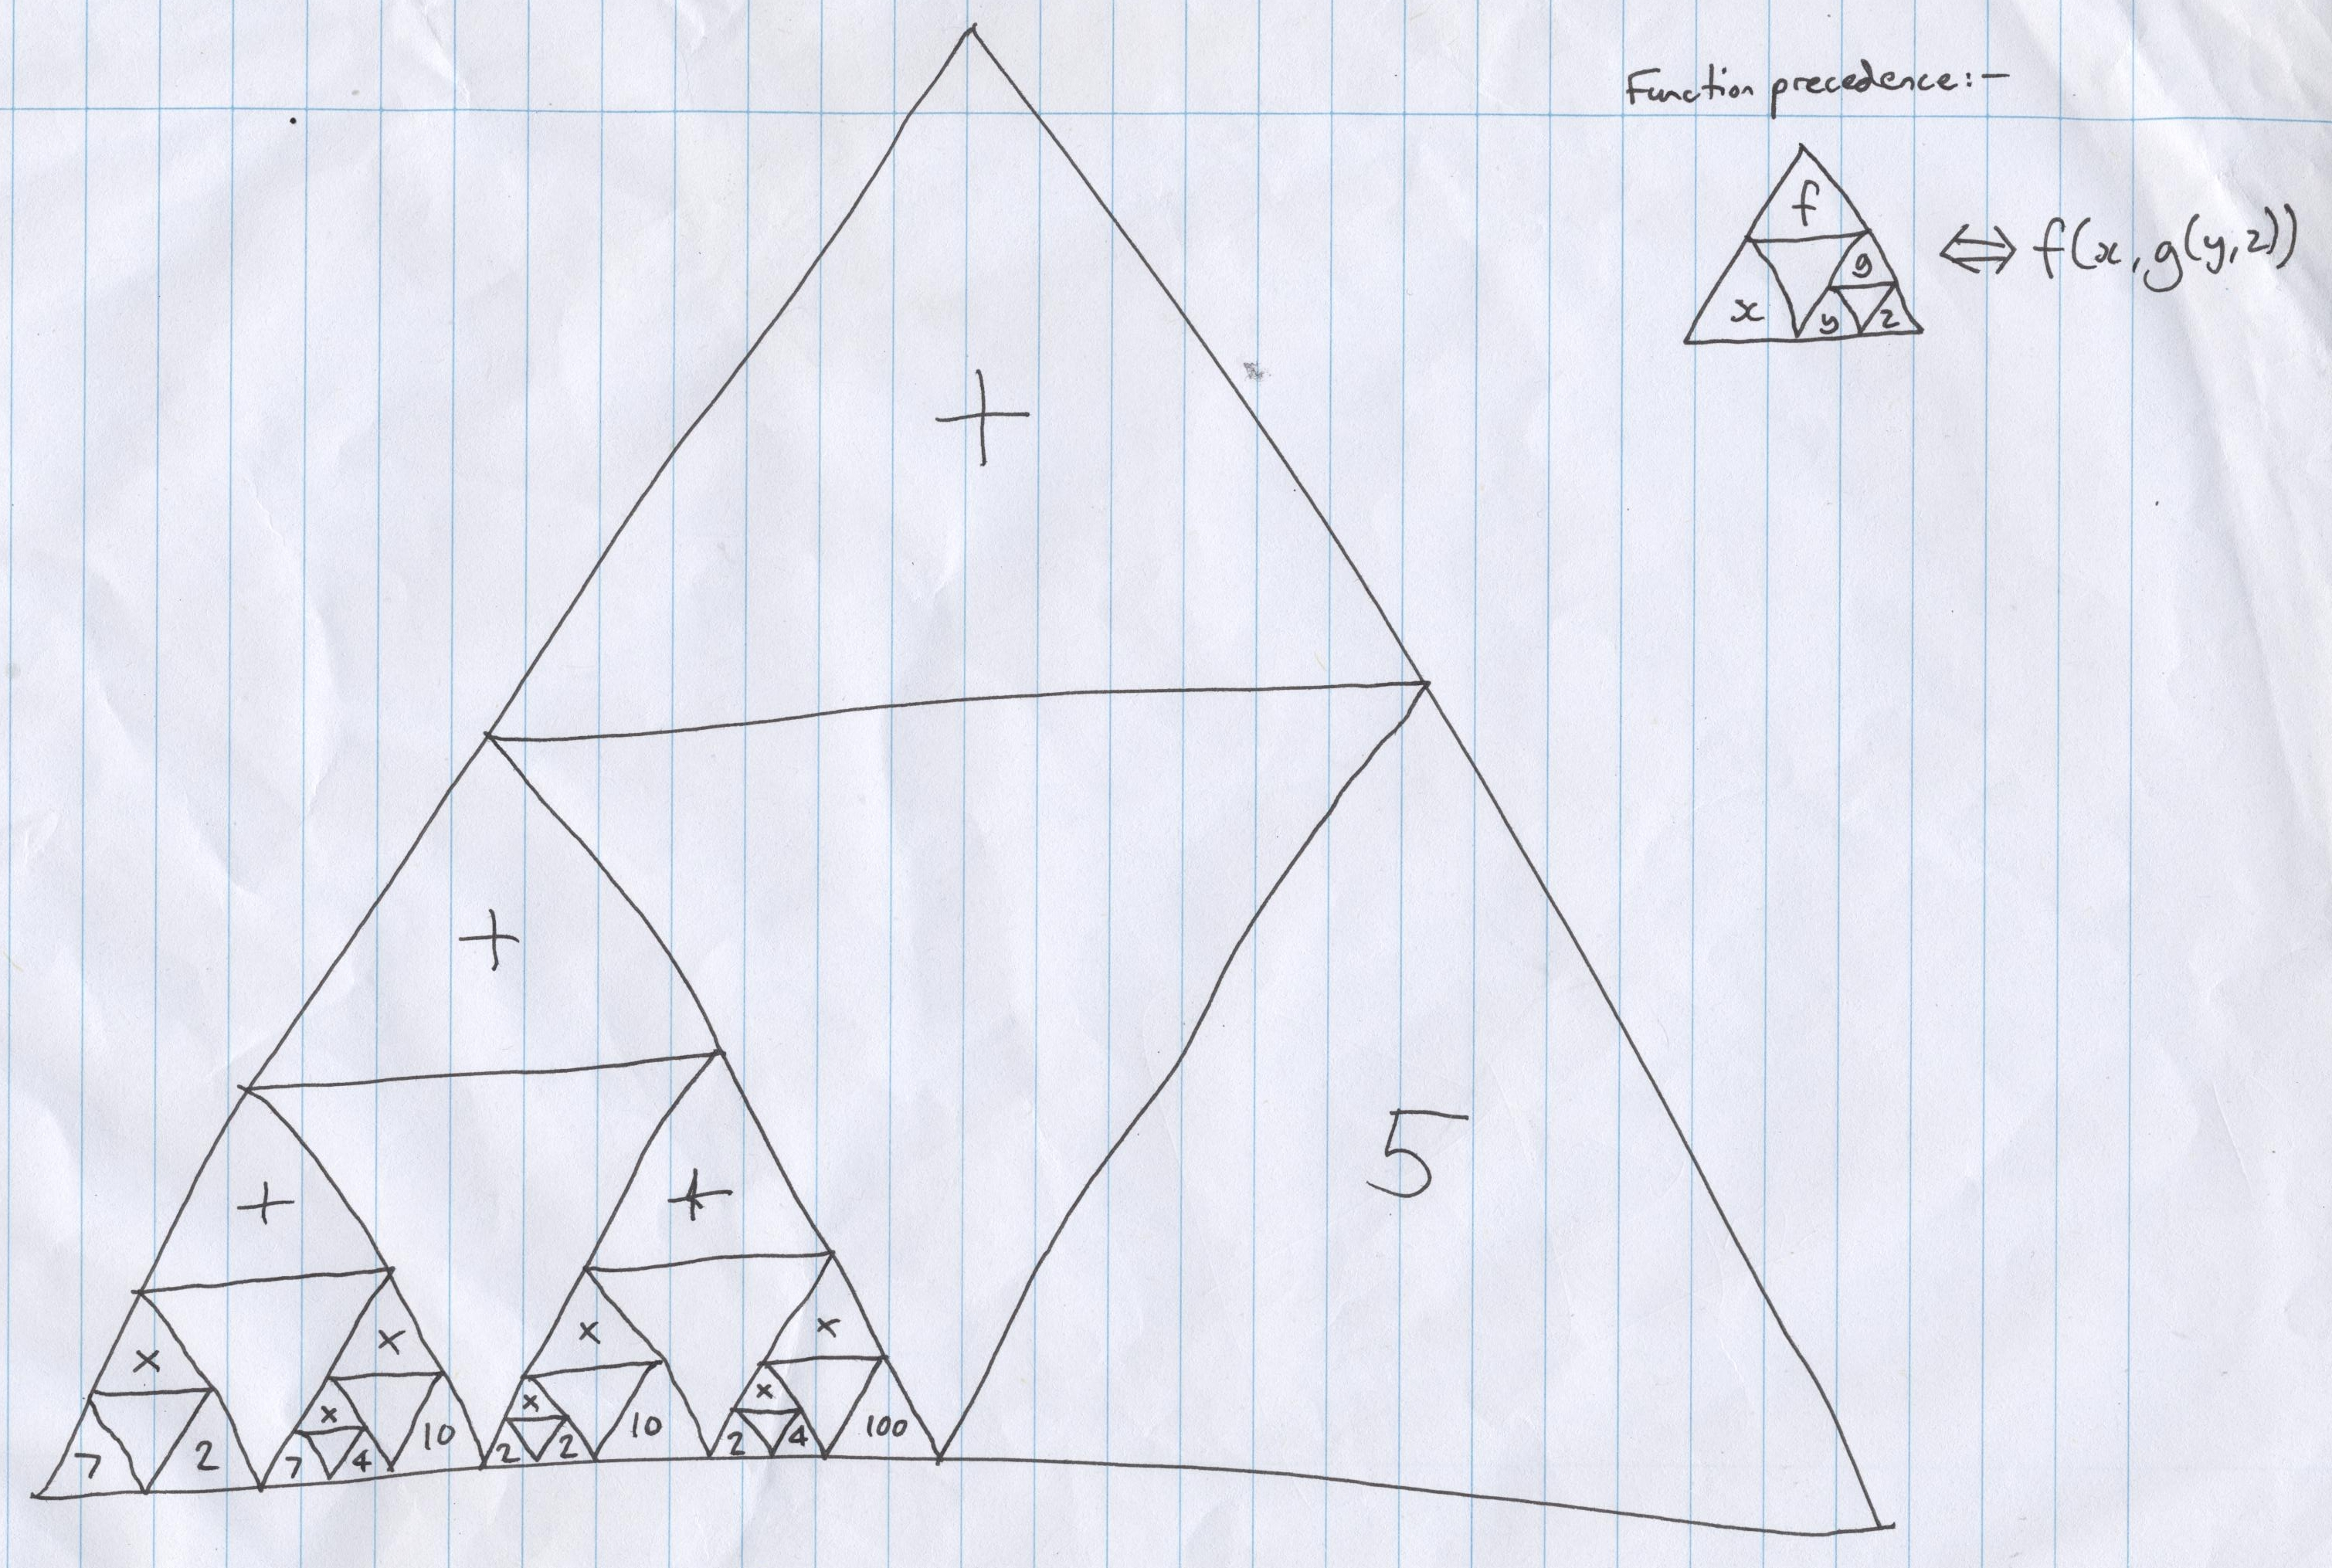
\includegraphics[width=\textwidth]{figs/mockups/sketches/31/31a.jpg}
\end{center}
\caption{A more refined sketch of a triangle-based language.}
\end{figure}
\end{center}

% \newpage

% \paragraph{Circles}\hfill

\begin{center}
\begin{figure}[H]
% \begin{wrapfigure}{r}{0.5\textwidth}
\begin{center}
\subfloat[]{
\parbox{4cm}{
\begin{center}
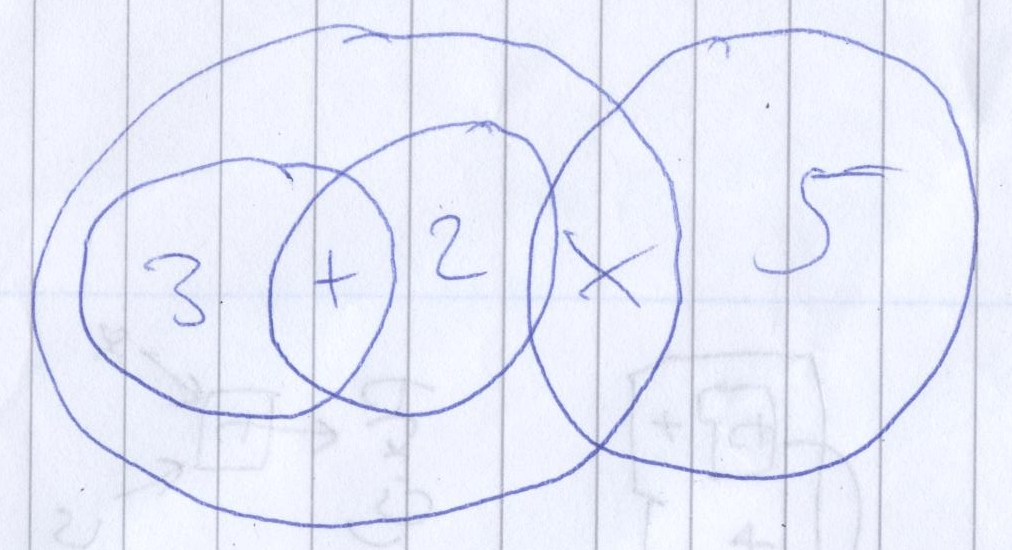
\includegraphics[width=4cm]{figs/mockups/sketches/12/12a.jpg}
\end{center}}}
\subfloat[]{
\parbox{4cm}{
\begin{center}
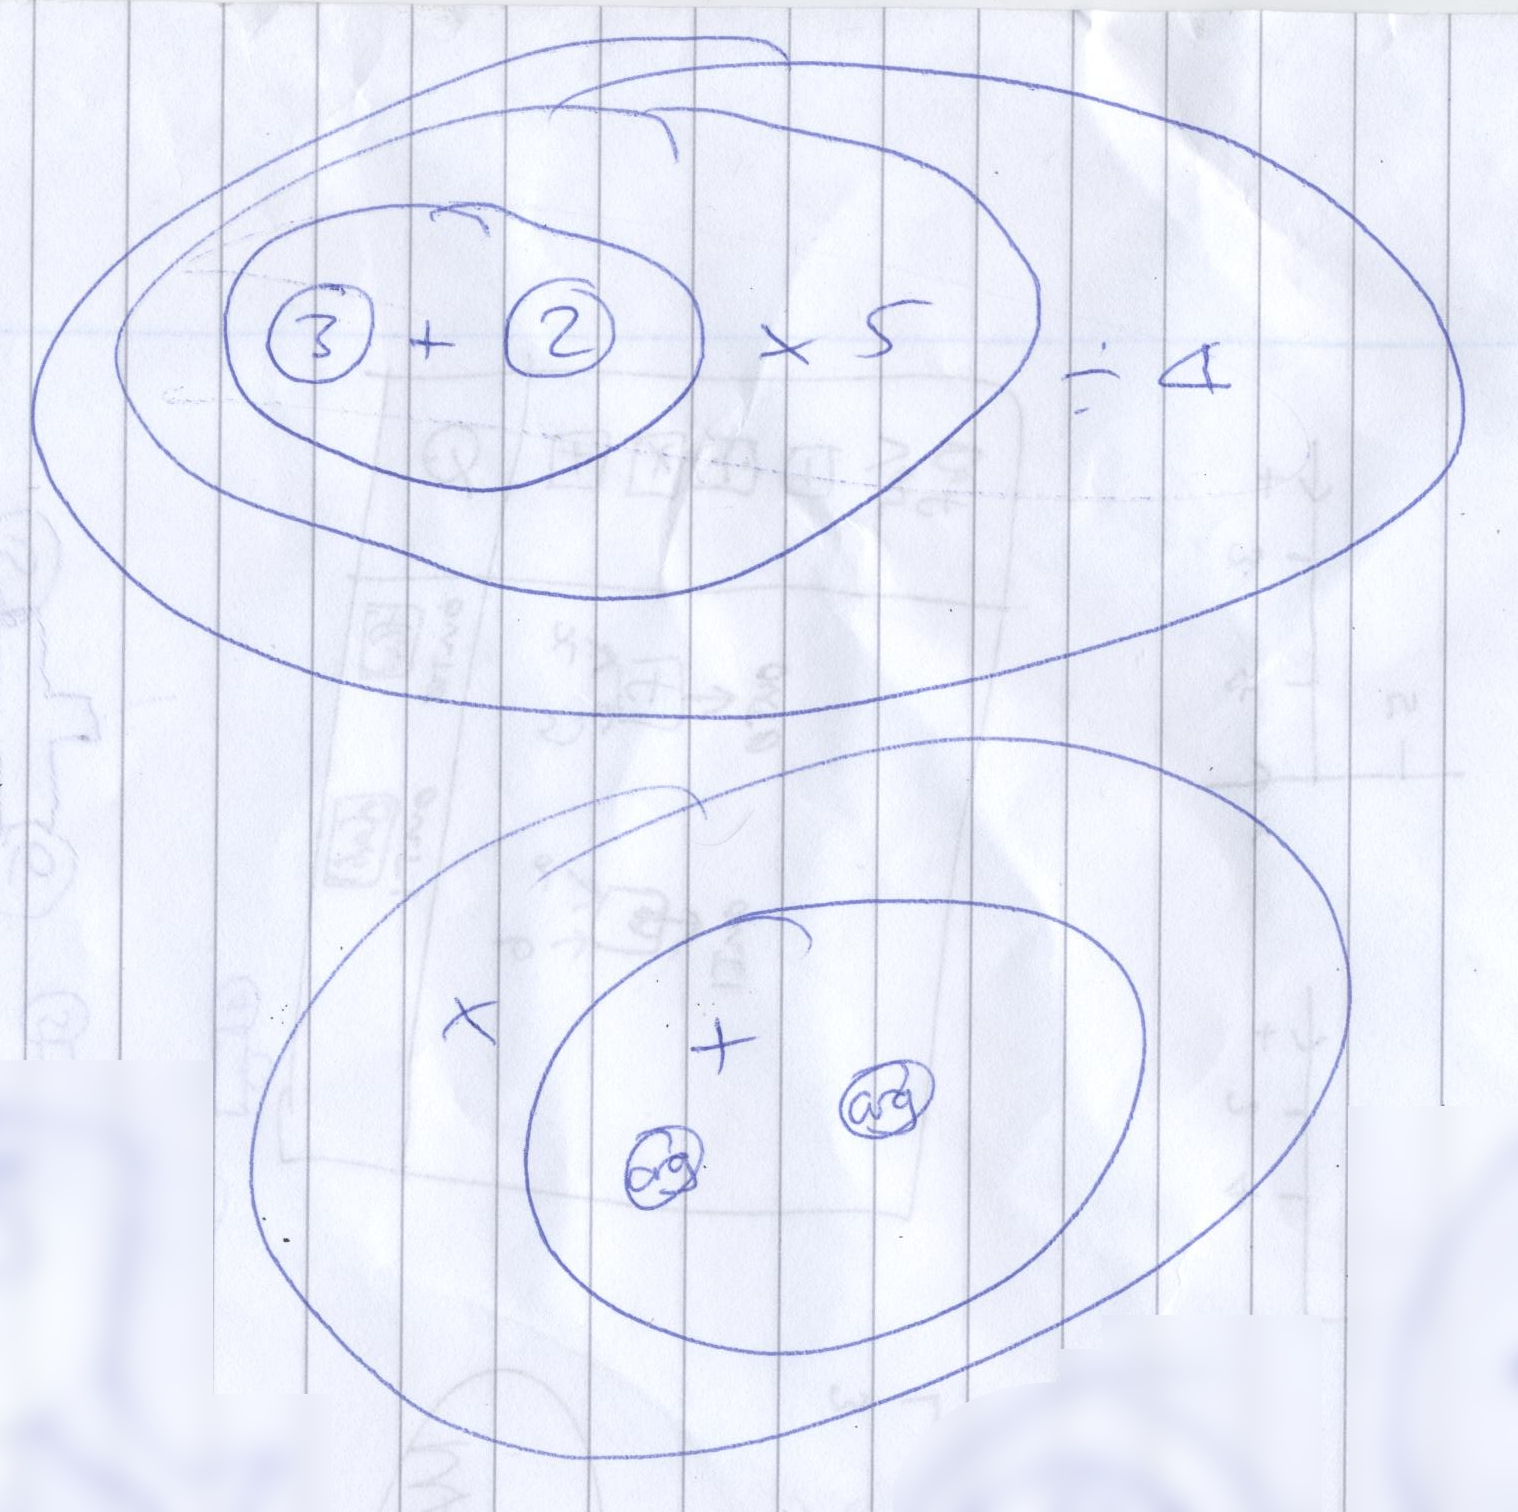
\includegraphics[width=4cm]{figs/mockups/sketches/12/12b.jpg}
\end{center}}}
\subfloat[]{
\parbox{4cm}{
\begin{center}
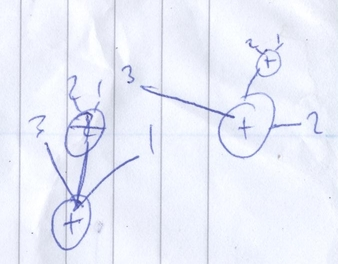
\includegraphics[width=4cm]{figs/mockups/sketches/12/12c.jpg}
\end{center}}}
\subfloat[]{
\parbox{4cm}{
\begin{center}
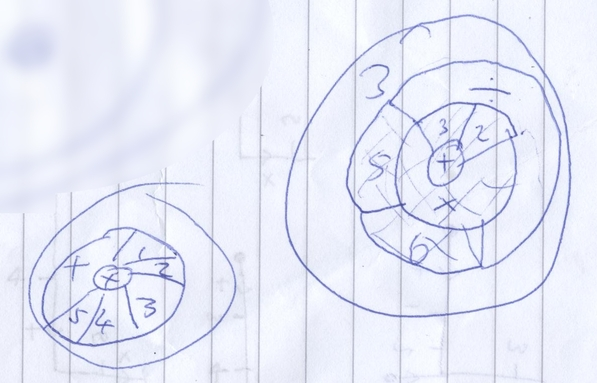
\includegraphics[width=4cm]{figs/mockups/sketches/12/12f.jpg}
\end{center}}}\\
\subfloat[]{
\parbox{4cm}{
\begin{center}
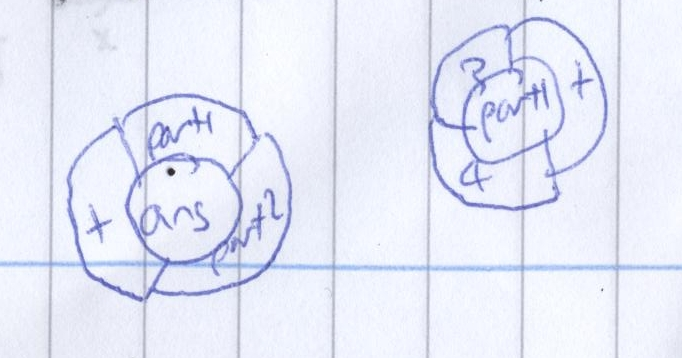
\includegraphics[width=4cm]{figs/mockups/sketches/12/12h.jpg}
\end{center}}}
\subfloat[]{
\parbox{4cm}{
\begin{center}
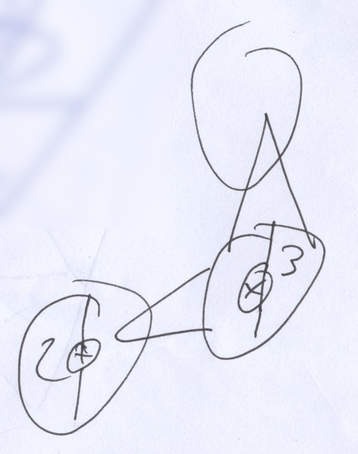
\includegraphics[width=4cm]{figs/mockups/sketches/41/41a.jpg}
\end{center}}}
\subfloat[]{
\parbox{4cm}{
\begin{center}
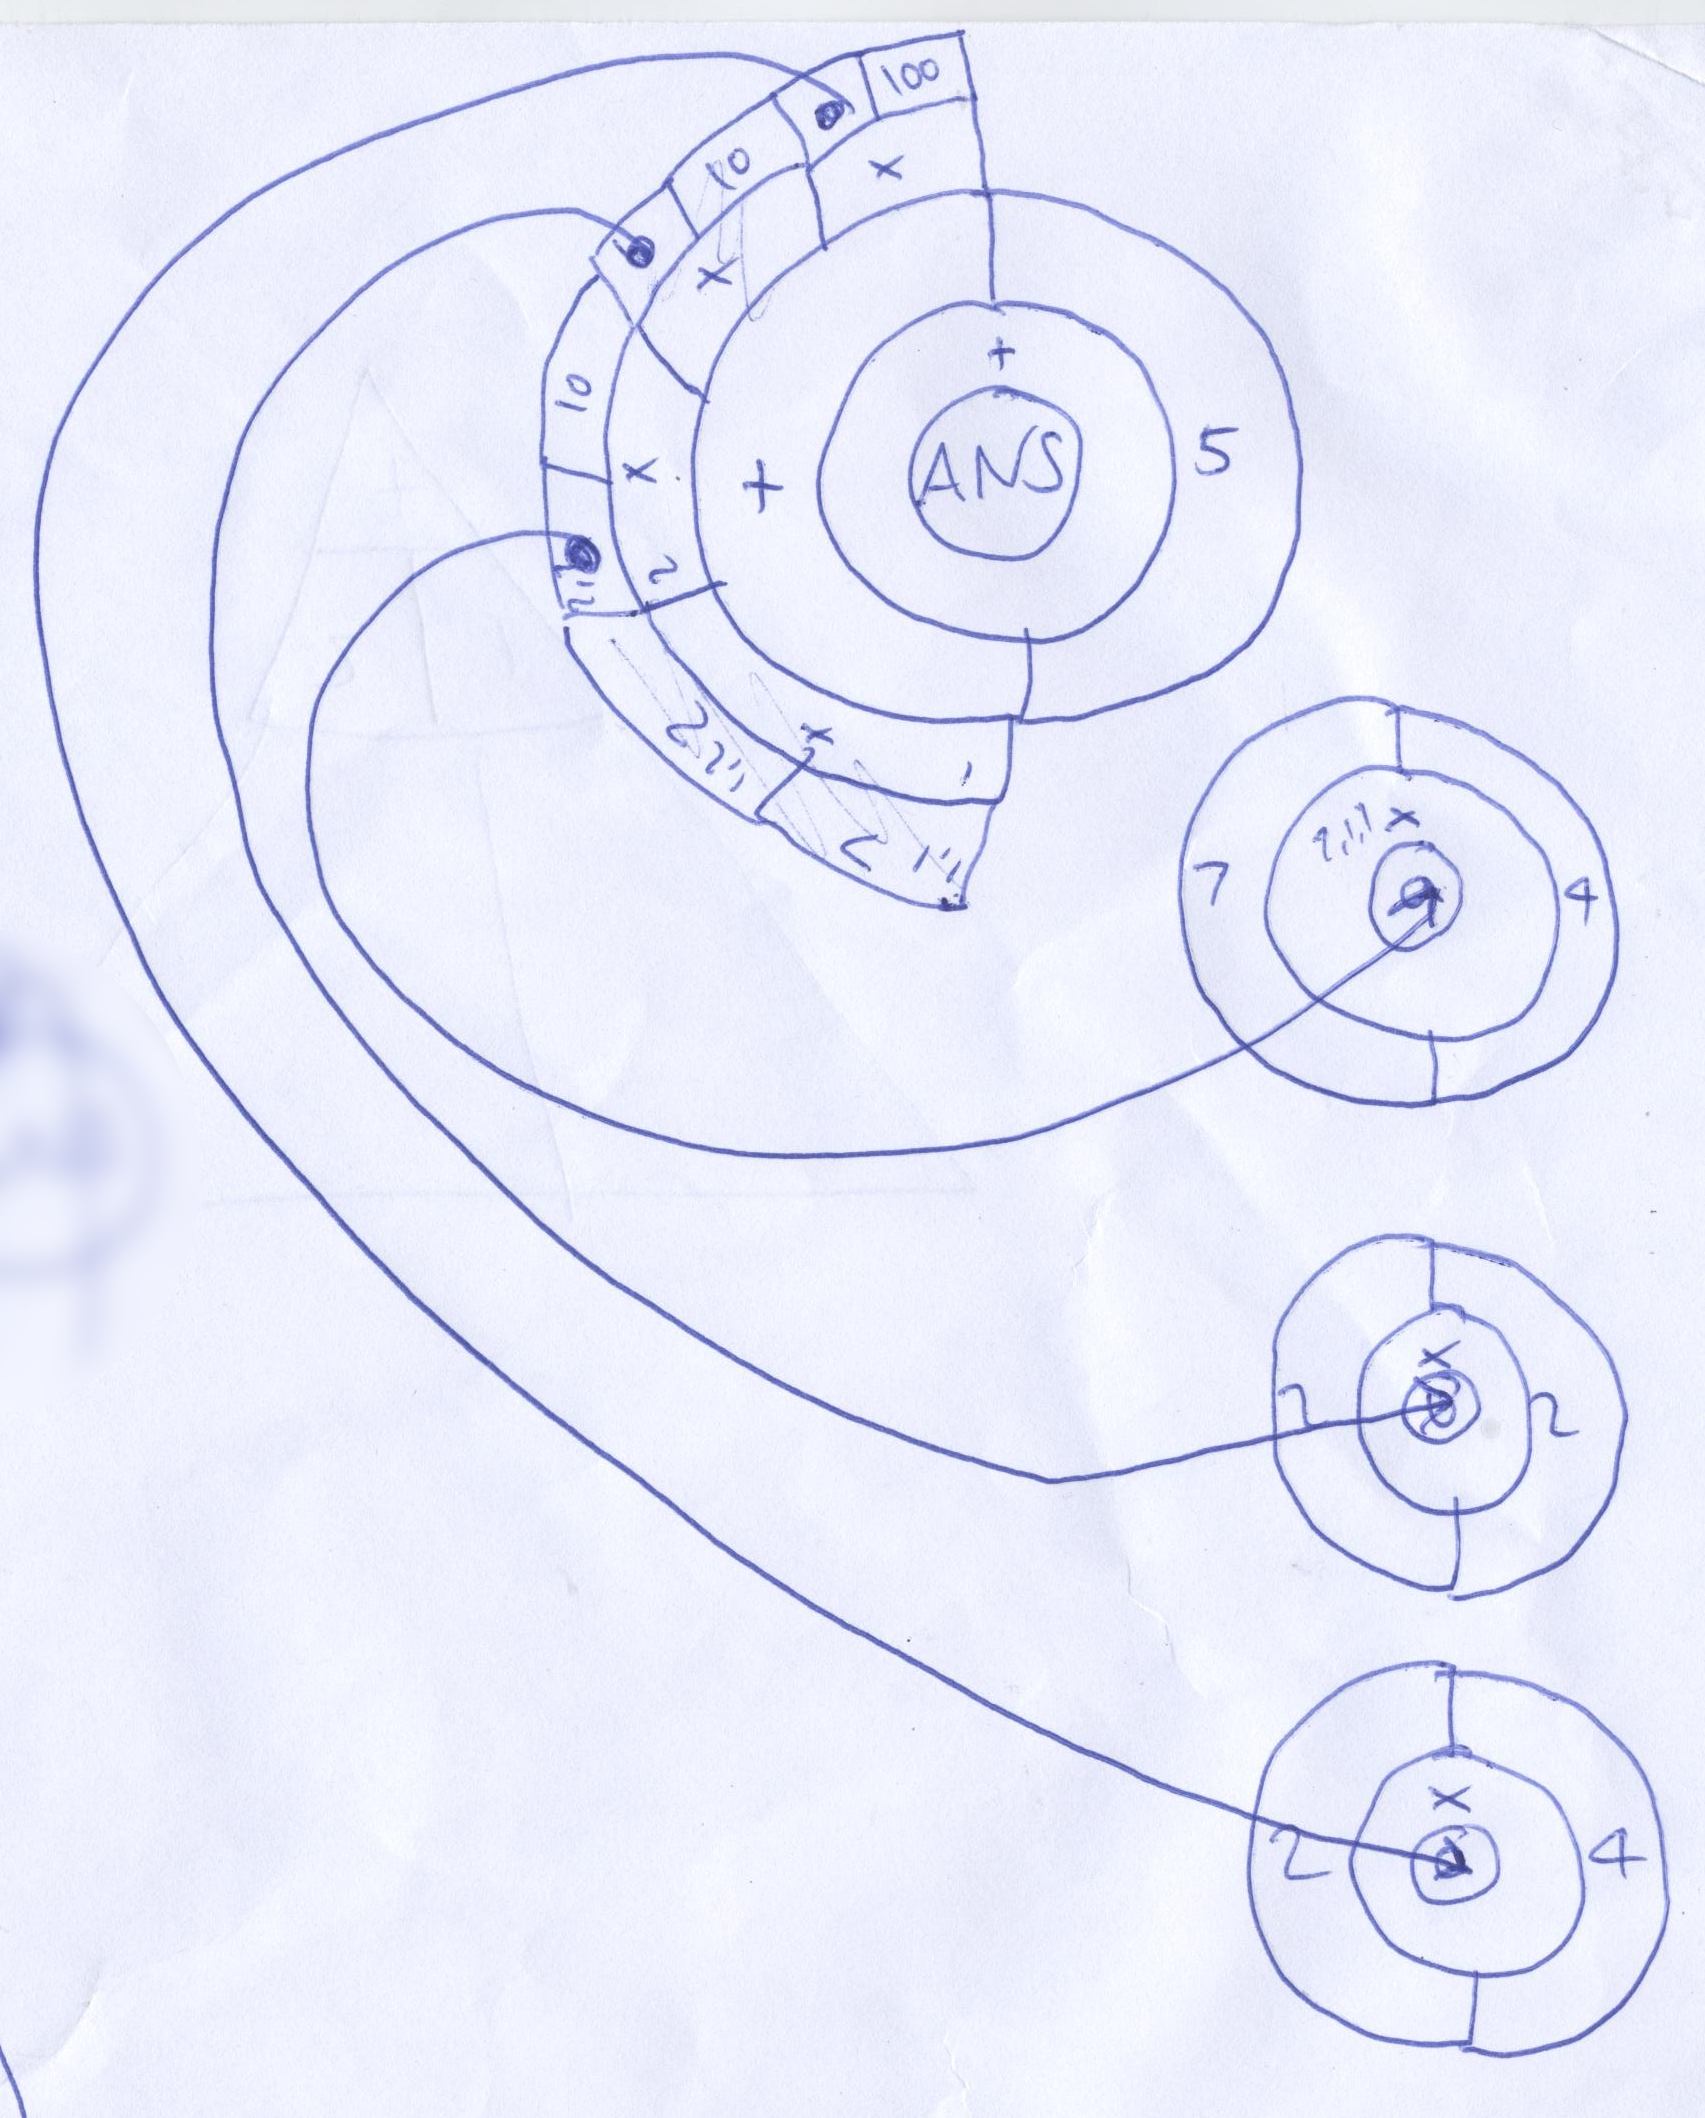
\includegraphics[width=4cm]{figs/mockups/sketches/41/41b.jpg}
\end{center}}}
\end{center}
\caption{Early designs for circle-based calculation metaphors.}
% \end{wrapfigure}
\end{figure}
\end{center}

\begin{center}
\begin{figure}
\begin{center}
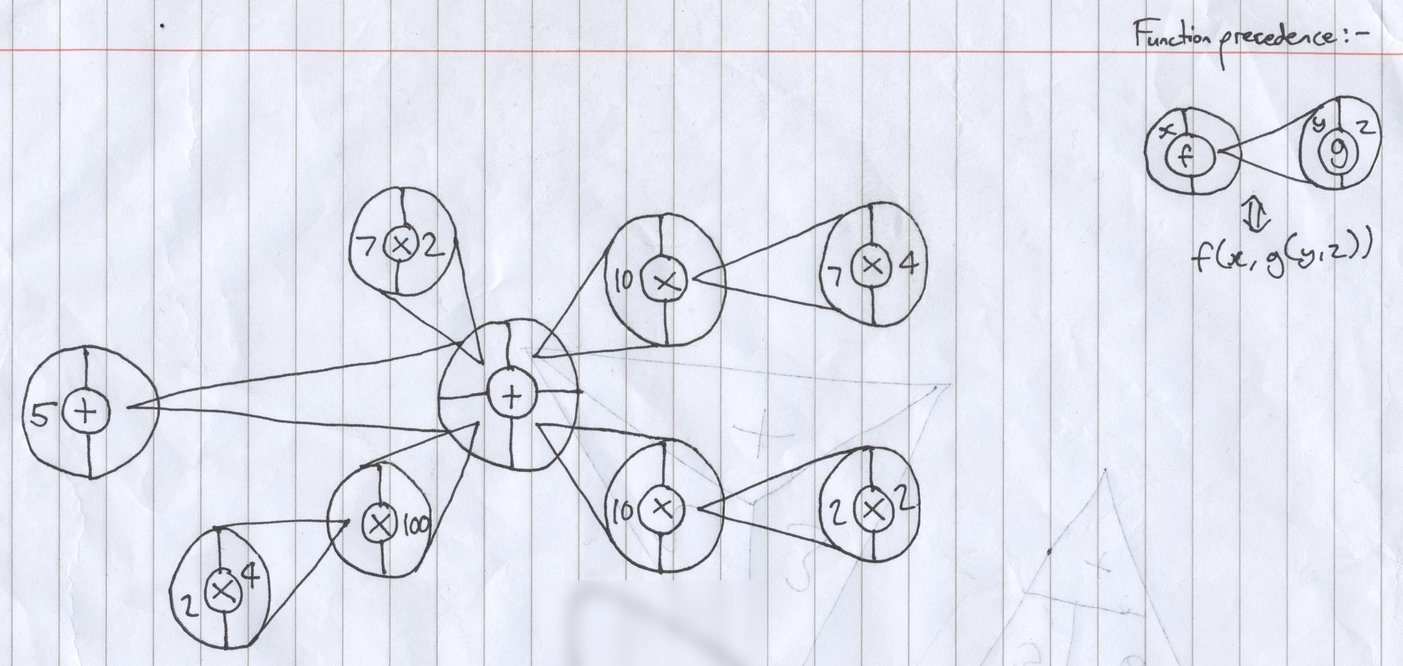
\includegraphics[width=\textwidth]{figs/mockups/sketches/21/21a.jpg}
\end{center}
\caption{A more refined sketch of a circle-based language.}
\end{figure}
\end{center}

% \newpage

% \paragraph{Other}\hfill

\begin{center}
\begin{figure}[H]
% \begin{wrapfigure}{r}{0.5\textwidth}
\begin{center}
\subfloat[]{
\parbox{4cm}{
\begin{center}
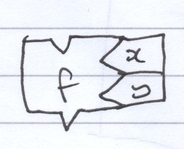
\includegraphics[width=4cm]{figs/mockups/sketches/11/11c.jpg}
\end{center}}}
\subfloat[]{
\parbox{4cm}{
\begin{center}
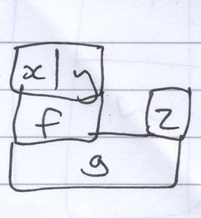
\includegraphics[width=4cm]{figs/mockups/sketches/11/11d.jpg}
\end{center}}}
\subfloat[]{
\parbox{4cm}{
\begin{center}
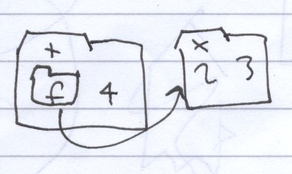
\includegraphics[width=4cm]{figs/mockups/sketches/11/11e.jpg}
\end{center}}}\\
\subfloat[]{
\parbox{4cm}{
\begin{center}
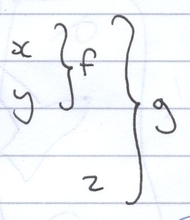
\includegraphics[width=4cm]{figs/mockups/sketches/11/11f.jpg}
\end{center}}}
\subfloat[]{
\parbox{4cm}{
\begin{center}
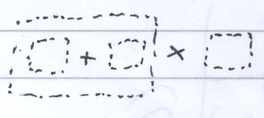
\includegraphics[width=4cm]{figs/mockups/sketches/11/11g.jpg}
\end{center}}}
\subfloat[]{
\parbox{4cm}{
\begin{center}
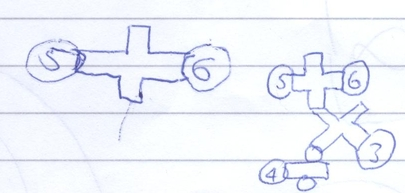
\includegraphics[width=4cm]{figs/mockups/sketches/11/11h.jpg}
\end{center}}}
\end{center}
\end{figure}
\newpage
\begin{figure}
\ContinuedFloat
\begin{center}
\subfloat[]{
\parbox{4cm}{
\begin{center}
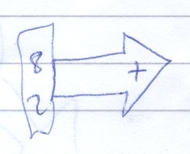
\includegraphics[width=4cm]{figs/mockups/sketches/11/11i.jpg}
\end{center}}}
\subfloat[]{
\parbox{4cm}{
\begin{center}
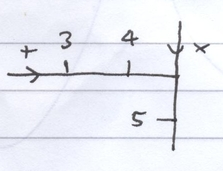
\includegraphics[width=4cm]{figs/mockups/sketches/11/11k.jpg}
\end{center}}}
\subfloat[]{
\parbox{4cm}{
\begin{center}
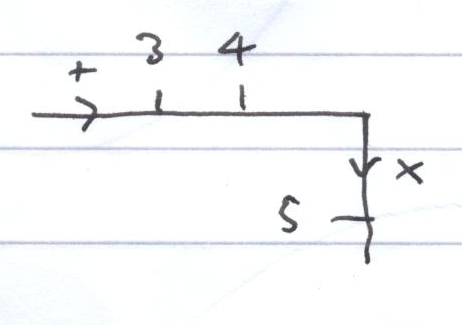
\includegraphics[width=4cm]{figs/mockups/sketches/11/11li.jpg}
\end{center}}}\\
\subfloat[]{
\parbox{4cm}{
\begin{center}
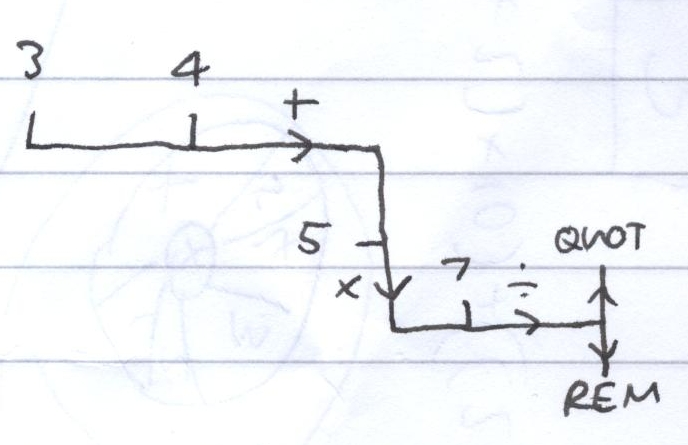
\includegraphics[width=4cm]{figs/mockups/sketches/11/11lii.jpg}
\end{center}}}
\subfloat[]{
\parbox{4cm}{
\begin{center}
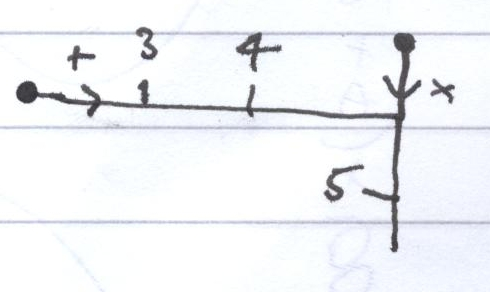
\includegraphics[width=4cm]{figs/mockups/sketches/11/11m.jpg}
\end{center}}}
\subfloat[]{
\parbox{4cm}{
\begin{center}
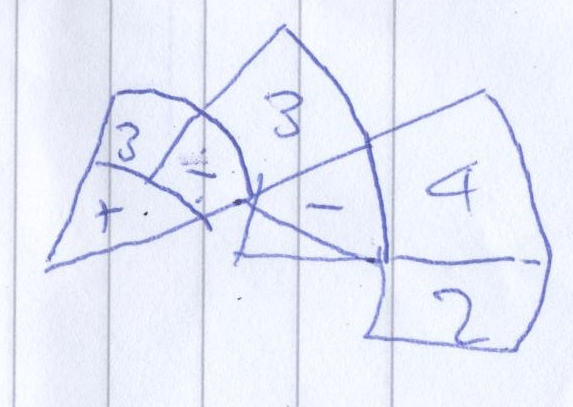
\includegraphics[width=4cm]{figs/mockups/sketches/12/12d.jpg}
\end{center}}}\\
\subfloat[]{
\parbox{4cm}{
\begin{center}
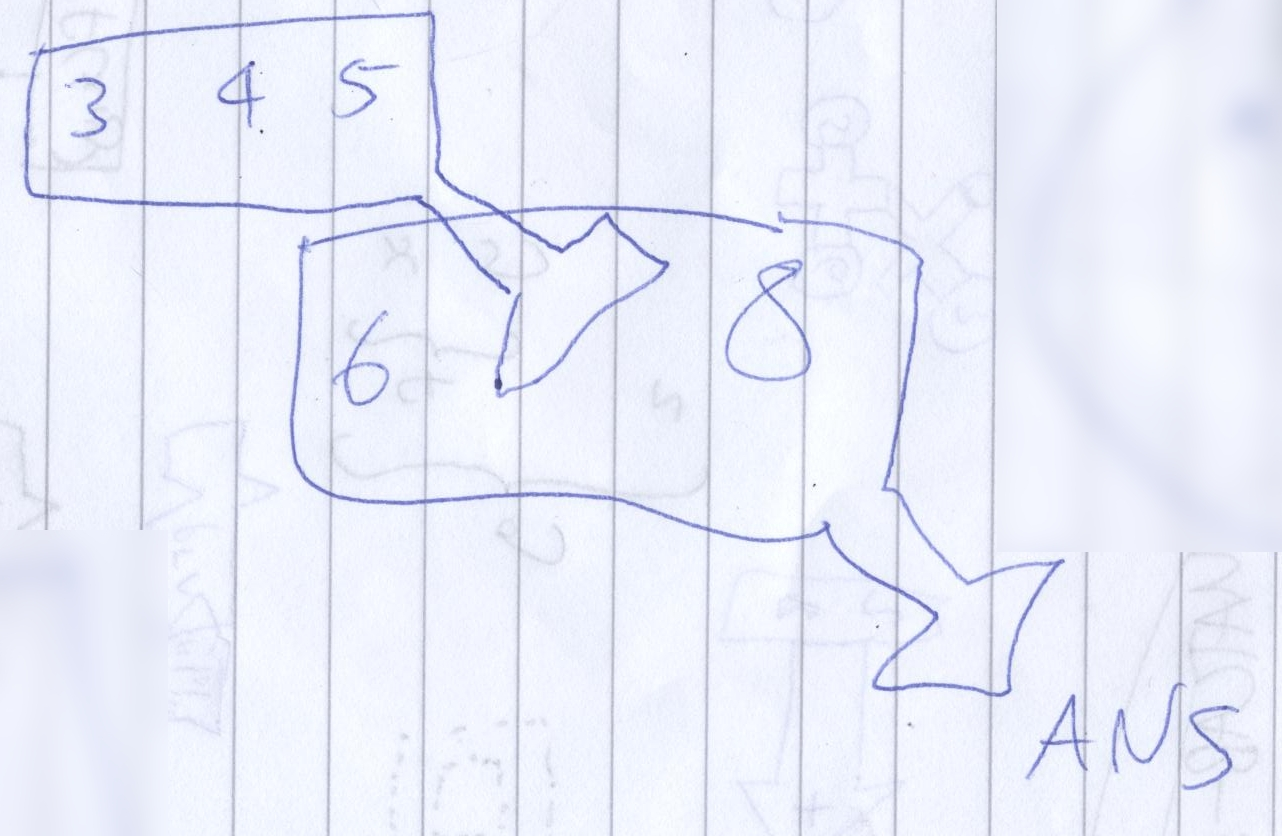
\includegraphics[width=4cm]{figs/mockups/sketches/12/12e.jpg}
\end{center}}}
\end{center}
\caption{Assorted early designs for other calculation metaphors.}
% \end{wrapfigure}
\end{figure}
\end{center}

\begin{center}
\begin{figure}[H]
\begin{center}
\subfloat[]{
\parbox{4cm}{
\begin{center}
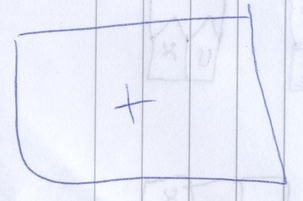
\includegraphics[width=4cm]{figs/mockups/sketches/12/12gi.jpg}
\end{center}}}
{\Huge $ \rightarrow $}% arrow
\subfloat[]{
\parbox{4cm}{
\begin{center}
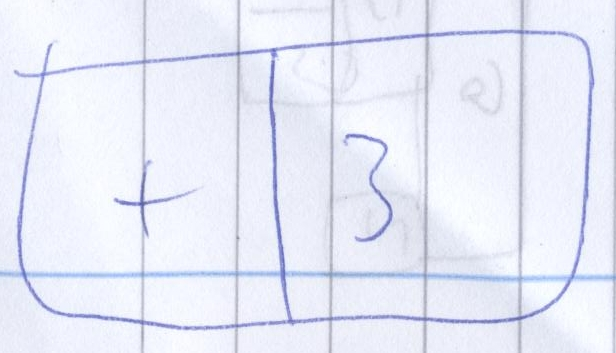
\includegraphics[width=4cm]{figs/mockups/sketches/12/12gii.jpg}
\end{center}}}
{\Huge $ \rightarrow $}\\% arrow
\subfloat[]{
\parbox{4cm}{
\begin{center}
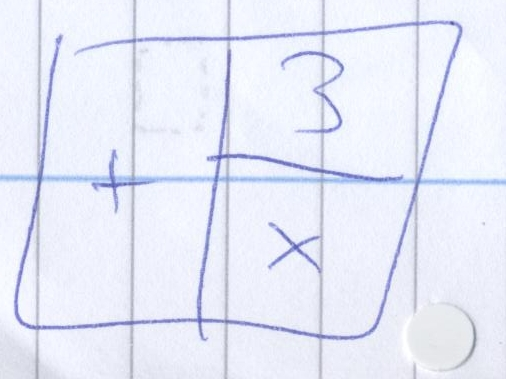
\includegraphics[width=4cm]{figs/mockups/sketches/12/12giii.jpg}
\end{center}}}
{\Huge $ \rightarrow $}% arrow
\subfloat[]{
\parbox{4cm}{
\begin{center}
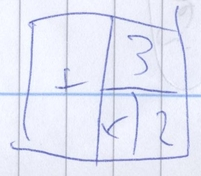
\includegraphics[width=4cm]{figs/mockups/sketches/12/12giv.jpg}
\end{center}}}
{\Huge $ \rightarrow $}% arrow
\subfloat[]{
\parbox{4cm}{
\begin{center}
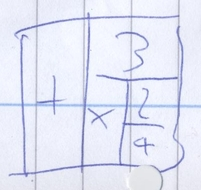
\includegraphics[width=4cm]{figs/mockups/sketches/12/12gv.jpg}
\end{center}}}
\end{center}
\caption{A sample progression of a calculation in a language based around infinitely halving a rectangle.}
\end{figure}
\end{center}

% \newpage

% \subsubsection{Preliminary Designs}
\subsubsection{Detailed Mockups}
% examples done using that prototyping software - balsamiq mockups
% draft designs on pwf

Some preliminary designs for the application and graphical language follow,
being more mature versions of three of the low-fidelity prototypes presented
above.  First is a combined flowgraph representation and
Read-Evaluate-Print-Loop (REPL) design.  The second design uses the Sierpiński
triangle as a basis for the visual metaphor.  The final design is the
circle-based language that eventually became the foundation for the rest of the
project.

\paragraph{Flowgraph Metaphor}\hfill

\begin{figure}[H]
\begin{center}
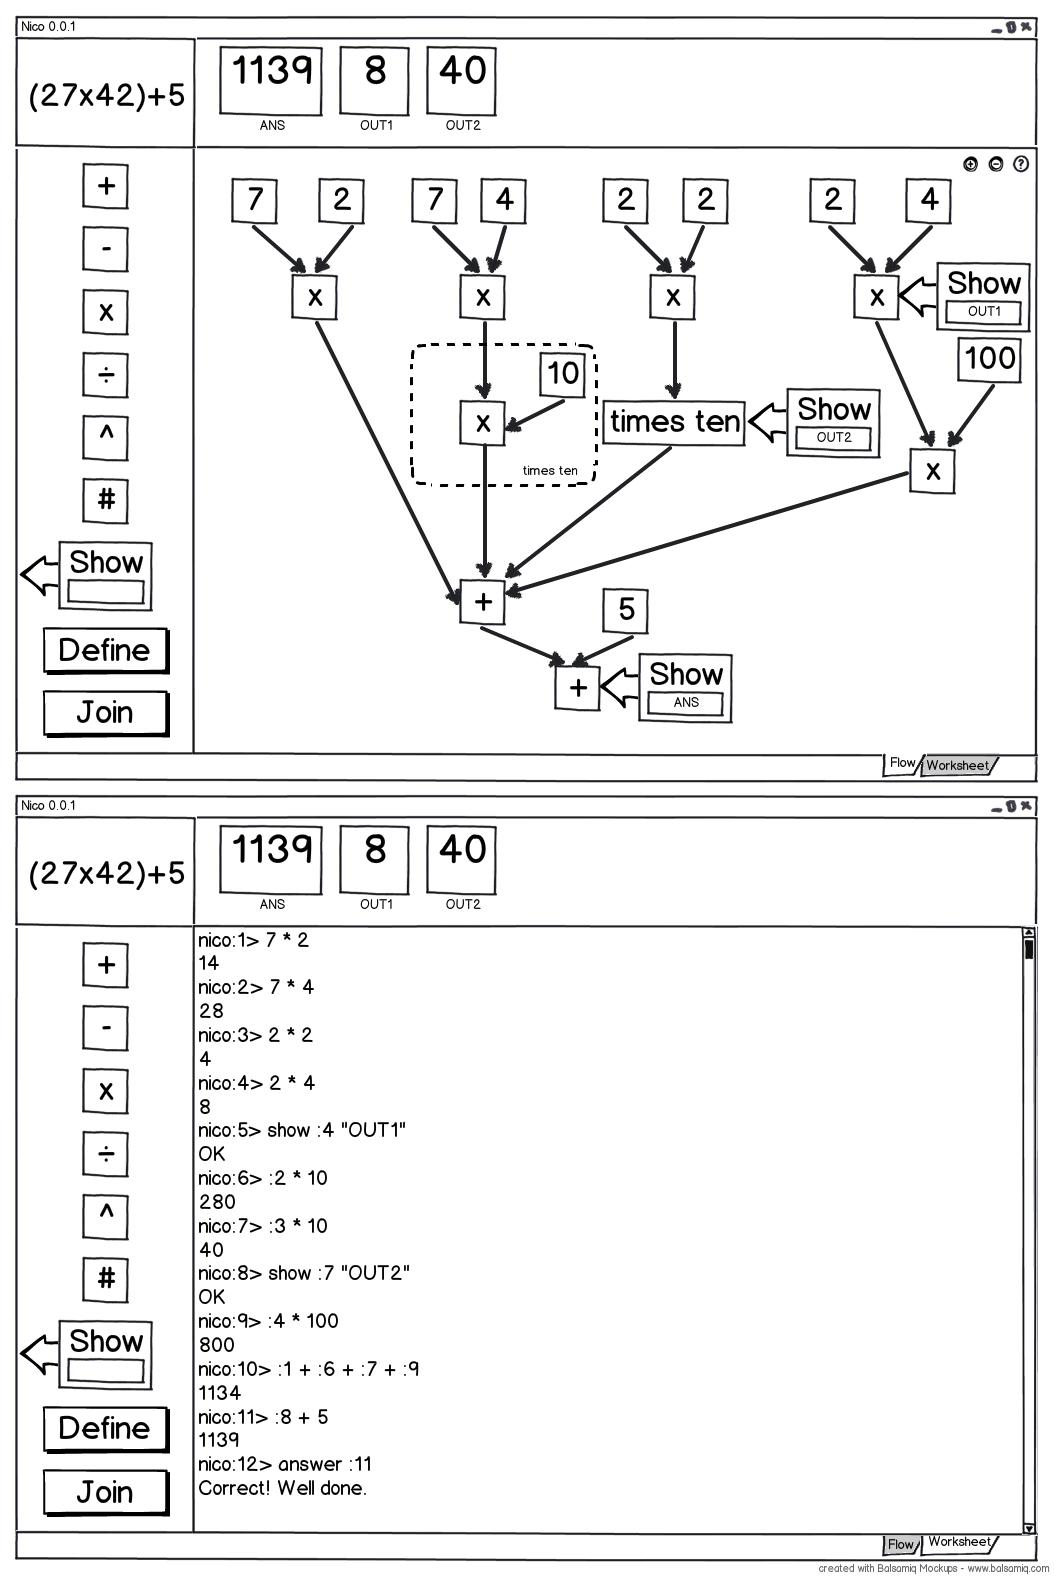
\includegraphics[width=\textwidth-4cm]{figs/mockups/flowgraph/img/fg-000.jpg}
\caption{The prototype flowgraph-style language.}
\end{center}
\end{figure}

The flowgraph idea initially outlined in the project proposal and included in
the low-fidelity prototypes above appears here as a more mature, revised
prototype, showing two screens of a sample application.  The top screen shows
the proposed application manipulating the graphical language, whilst the bottom
screen shows a REPL utilising a simple text-based language for users more
comfortable with writing than the visual metaphor.

% TODO: add scroll bar to box selection panel?  have claimed that it's scrollable but it's not showing it!
% TODO: similarly for the canvas
The application is comprised of one window containing several panels.  The
current question being answered is displayed in the top left-hand corner.
Below this, a scrollable panel running down the left side of the window
contains the fundamental components of the notation: boxes representing numbers
and operations, both provided and user-defined, with two buttons below to
change the action of clicking the mouse (explained in greater detail below).  A
panel that runs along the top of the window contains output boxes, areas that
display the result of a calculation at a user-determined point in the
application.  Further boxes appear here as the user demands them, by using the
{\sfapp Show} function.  The {\sfapp ANS} box is a specialised case of this,
which displays what the user currently wishes to submit as the answer to the
question.  The canvas panel occupies the majority of the window, and this is
the area in which the answer is constructed using the various components of the
graphical language.  In the top right-hand corner of the canvas are three
buttons, to zoom in and out of the current calculation and to bring up a help
window.  For especially large or zoomed-in calculations, the canvas is
scrollable.  At the bottom of the window are two tabs, {\sfapp Flow} and
{\sfapp Worksheet}.  When {\sfapp Flow} is selected, the graphical language is
available for use in answering the question.  When {\sfapp Worksheet} is
selected, the user is able to use a simple textual language in a REPL to answer
the question.

Of all the prototypes shown here, this version of the graphical language is the
most like a traditional programming language, in that it allows the user to
define reusable functions, and includes functionality similar to print
statements.  The icons at the side of the application are used to select the
desired function, from a set that includes addition, subtraction,
multiplication, division, exponentiation, number input, {\sfapp Show},
{\sfapp Define} and {\sfapp Join}.  Addition, subtraction, multiplication,
division and exponentiation are all dragged-and-dropped from the icons at the
side to a point on the canvas, causing a box containing their respective
functions to appear at that point.  Number input ({\sfapp \#}) is similar, but
the user inputs a number using the keyboard after the box is created.  The box
then contains that number.  {\sfapp Show} displays the output of the junction to
which its arrow points, in the output box at the top of the screen with the label
input by the user after placing it.  If the box with the label does not yet
exist, it is created next to the existing output boxes.  {\sfapp Define} and
{\sfapp Join} are not boxes to be dragged-and-dropped; they are modes of
operation.  When {\sfapp Define} is activated, dragging the mouse on the canvas
draws a box around sections of the diagram -- the user is able to define
functions by doing so, and by providing a label for the section of diagram that
has been highlighted, a corresponding box can be dragged-and-dropped from the
list of icons (as show in \emph{Fig. 2.2} with the {\sfapp times ten}
function).  When {\sfapp Join} is active, dragging between two points on the
canvas creates an arrow between them that means that the source of the arrow is
used as an argument to the destination of the arrow.  In defining functions,
if arrows cross the boundary of the definition box and they are incoming, input
is required to future uses of the function.  One outgong arrow is allowed to
indicate the output of the function.  Using this notation, answers are submitted
by {\sfapp Show}ing the output at a point in the calculation to the output box
{\sfapp ANS}.

This particular graphical language tries to have a very high visibility,
minimising the number of hidden dependencies between calculations by making
every connection explicit: as a dataflow representation of a calculation
\cite{Blackwell1998}, the flow of information through the diagram is made very
clear.  This language is considerably less viscous than the handwritten method,
as it is trivial (albeit not demonstrated in \emph{Fig. 2.2}) to remove and
replace a box or arrow in the diagram, as opposed to writing out a new set of
calculations or replacing several instances of a component by crossing them
out.  Each box is able to be relocated on the canvas, increasing the
juxtaposability of the system, and the user is able to define their own
abstractions.

The textual language improves upon the traditional means of handwriting
arithmetic by revealing otherwise-hidden dependencies using references to line
numbers.  As the target audience is not yet required to have formally learnt
(or, indeed, encountered) algebra, this notation includes a function \verb¬:¬,
which takes a single number \emph{n} as an argument and returns the result of the
calculation performed on line \emph{n}.  Answers are submitted using a function
\verb¬answer¬ that takes a single number (shown here using a line reference that
is resolved to a number) as an argument.  Other functions include addition,
subtraction, multiplication, division and exponentiation, all of which take two
or more numerical arguments and are used in the familiar infix form.  A function
\verb¬define¬ is also included, although not shown here.  Finally, there is the
\verb¬show¬ function, which behaves similarly to a print statement.  It takes a
numerical argument \emph{n} followed by a string argument \verb¬str¬, and
displays \emph{n} in the output box named \verb¬str¬ at the top of the screen.
If there exists no such output box, it is created next to the existing boxes.
Note that \verb¬answer n¬ is logically equivalent to \verb¬show n "ANS"¬; the
\verb¬answer¬ function was included here to increase clarity.

This design was abandoned as it was deemed to be too complex for the target
audience (Year 5).  The intention of this project is not to implement yet
another programming language for learners, and by providing features like the
REPL and function definition, the system unnecessarily overprovides.  In
addition to this, the flowgraph representation had a number of shortcomings.
For example, it is not immediately clear in what order the arguments feed into
an operation, which is confusing for non-commutative functions such as
subtraction.  Furthermore, the language is quite verbose.  Although this is not
inherently a disadvantage, a more compact representation would be preferable,
in order to make expressions written in the notations more readable to people
other than the author.

\paragraph{Sierpiński Triangle Metaphor}\hfill

\begin{figure}[H]
\begin{center}
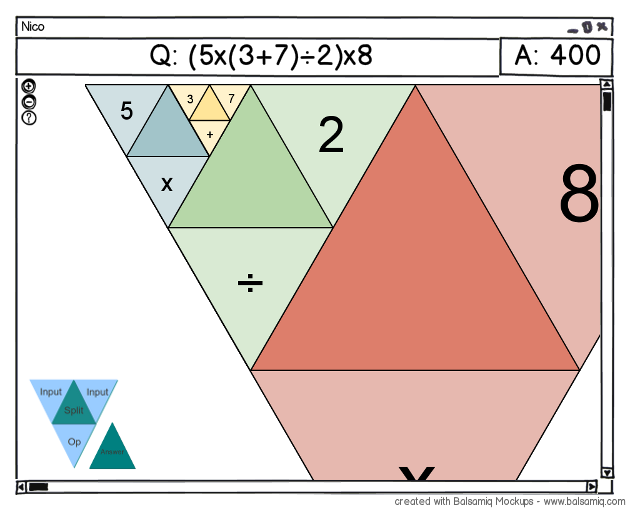
\includegraphics[width=\textwidth]{figs/mockups/sierp/sierp_mockup_full.png}
\caption{The prototype Sierpiński-triangle-based language.}
\end{center}
\end{figure}

This prototype uses a zooming instance of the Sierpiński triangle fractal as
the basis of its notation.  It is shown here manipulating a simple calculation.

The application consists of a single window containing two panels and a canvas
area.  The right-hand panel displays the current total of the calculation,
and the other panel displays the question currently being answered.  In the
canvas area, there are buttons for zooming in and out, a help button and
buttons controlling the composition of structures within the language.  When a
triangle has been selected by clicking on it, clicking the {\sfapp Op} button
presents the user with a choice of operations (namely +, -, × and ÷) to use in
the bottom segment of the triangle.  Clicking either of the {\sfapp Input}
buttons allows the user to input a value into their respective sections, and
clicking on the {\sfapp Split} button creates a new triangle expression within
the left-hand triangle.

This notational system is based around binary operations represented as the
component triangles of a Sierpiński fractal, the logic behind this being that
the fractal structure emphasises that each calculation is part of a larger
whole.  The notation is read by using the left and right sub-triangles as
arguments (left first, right second) to the operation in the bottom triangle.
The structure is colour-coded, such that each subexpression is a different
colour to its precedent superexpression.  This allows the user to abstract away
subexpressions as units to be manipulated as any other input to an operation
would be.  The hidden dependencies of the handwritten method are greatly
diminished in this manner, as viewing the internal structure of a
calculation's subexpressions is simply a matter of zooming-in to the
appropriate triangle.  Viscosity is also considerably reduced, as making a
change in one expression does not require the change to made anywhere else, as
the results of that expression are passed to the rest of the calculation.  This
does not completely remove viscosity, as a misresrepresented value still has to
be replaced several times if it appears in several different expressions, but
this is still an improvement over handwriting.  Indeed, the fact that
calculations are editable more than once, by virtue of using a computer rather
than paper, makes this less viscous than pen and paper.  The system is quite
visible, but has a very low juxtaposability, as all calculations are restricted
to their respective places in the triangle template.

This design was ultimately abandoned as it was deemed to be awkward for a
number of reasons, not least because it was based solely around binary
operations, meaning that to solve the simple question 1+2+3+4, one has to either
calculate ((1+2)+3)+4, which is inefficient, or mentally calculate that
1+2+3=6, and then calculate 6+4, which is obviously unacceptable for a system
that intends to help the user express themselves mathematically.  The severe
lack of juxtaposability is also a problem: as each expression must fit into the
larger structure, it is not possible to reorder them at will, without
fundamentally altering the calculation being performed.  It also enforces a
top-down approach to calculation: one is required by the system to begin with the
outermost calculation and work inwards.  There is no provision for putting a
larger triangle around an existing calculation.  In addition to this, a
somewhat-informal survey of potential notations was conducted, asking
approximately ten subjects to answer some sample questions in this notation and
the circle-based notation (below).  Subjects found this notation less clear,
and were much better able to complete questions correctly using the circle
notation.
% survey
% TODO: can't put subexpressions into right-hand triangle

% what/mockup
% application
% language
% abandoned

\paragraph{Circle Metaphor}\hfill

\begin{figure}[H]
\begin{center}
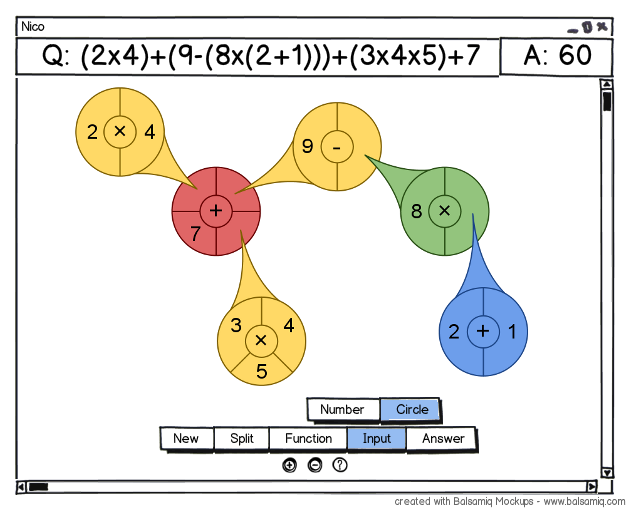
\includegraphics[width=\textwidth]{figs/mockups/circles/nico_circmock.png}
\caption{The prototype circle-based language.}
\end{center}
\end{figure}

This prototype uses a notation based around circles as individual units of
calculation, linked in such a way as to indicate the flow of information.
Although it is related to the flowgraph metaphor (above), it has a number of
key differences.

The application comprises, similarly to the Sierpiński model above, a single
window with two panels and a scrollable canvas area, with some buttons to
control the input of data.  The right-hand panel shows a running total of the
user's calculation, and the other panel shows the question currently being
answered.  The canvas area has three buttons at the bottom: zoom in, zoom out
and help.  The larger buttons above these control the action that clicking the
mouse on the canvas performs.  When {\sfapp New} is active, clicking on the
canvas creates a new circle at that location.  When {\sfapp Split} is active,
clicking on a circle increases the number of arguments it has (initially two,
up to a maximum of eight).  When {\sfapp Function} is selected, clicking on a
circle presents the user with a choice of +, -, × and ÷ to use as that circle's
operation.  When {\sfapp Input} is selected, as shown in \emph{Fig. 2.4}, the
user is presented with two further options, {\sfapp Number} and
{\sfapp Circle}.  When {\sfapp Number} is active, clicking on a circle's
argument allows the user to change the value of that argument.  When
{\sfapp Circle} is active, the user is able to click and drag from one circle
to an argument of another, indicating that they wish to use the results of one
circle's calculation as the argument to another circle's calculation.  Finally,
the {\sfapp Answer} button submits the current total as the answer to the
current question.

This notational system uses linked circles representing individual expressions
as its primary metaphor for constructing calculations.  It is similar to the
flowgraph metaphor presented above, except that instead of boxes for each
argument and operation all linked together, single, linkable objects in this
system are complete expressions, rather than components.  Also, there is only
one visible output, namely the overall result of the calculation as a whole.
As for the circles themselves, they consist of an operation at the centre,
orbited by arguments, which are evaluated clockwise from 0°.  Each argument can
either be a number or the tail of another circle, representing the result of
the calculation that that circle stands for.  The circles are colour-coded,
with each `layer' having its own colour.  In this case, the root circle is red,
the circles feeding directly into it are yellow, the circles feeding into those
circles are green and the circles feeding into those are blue.  It is possible
to move circles around the canvas by clicking and dragging them to the desired
location.  Compared to the handwritten approach, this notational system is much
more visible, and very much more juxtaposable, allowing the user to construct
the diagram in a way that is comfortable for them, and allowing them to compare
elements side-by-side if they need to.  Unlike with the Sierpiński metaphor,
the user is not restricted to one order or pattern of constructing a
calculation: calculations can be performed bottom-up, top-down or a mixture of
both, as is comfortable for the individual user.  The system of tails feeding
into other circles also makes the dataflow clear, eliminating many of the
hidden dependencies of handwritten calculation.  For similar reasons to the
flowgraph metaphor, the circle notation also reduces viscosity, as changing a
subexpression automatically alters all of its superexpressions.  Finally, the
system requires little premature commitment, as piece of the diagram can be
created, deleted and swapped in and out at will, so it is ideal for
exploration, allowing the user to try many ways of solving a problem within the
application, rather than having to use a secondary notation or device to help
work through a problem in a more familiar manner and then transcripting that
solution into the new notation.

This design was the one that was ultimately chosen as the basis for the project
as it neatly solved, or at least ameliorated, many of the problems listed with
handwritten arithmetic, without being too complex for the target audience (as
with the flowgraph system), and without being too restrictive with regard to
mathematical expression.  In addition to this, the results of the survey
mentioned above also indicated that people got on well with this notation; the
test subjects found it considerably easier to use than the Sierpiński notation,
and made fewer mistakes in handwriting this notation than the alternative.
% survey

% what/mockup
% application
% language
% chosen

% \section{Additional Tools}

% Luke's:
% Throughout the project, I developed additional support tools to assist with
% design, development and testing. These will be described at the relevant place
% in the implementation chapter.
% lol

% \subsection{Third-Party Tools}
\section{Third-Party Tools}

What follows is a list of the third-party tools that were used in the
development of the project.
\begin{itemize}
\item Ubuntu Linux 10.04, Arch Linux 2010.05, Microsoft Windows 7
\item Clojure 1.2.0
\item Leiningen 1.6.1.1
\item OpenJDK 6
\item Seesaw 1.3.1-SNAPSHOT
\item swank-clojure 1.3.4-SNAPSHOT
\item GNU Emacs 23.1.1
\item A modified version of Overtone's Emacs configuration \cite{OvertoneEmacsD}, including:--
\begin{itemize}
\item SLIME/SWANK (revision as of 15/10/2009)
\item clojure-mode 1.11.5
\item undo-tree 0.3.3
\end{itemize}
\item Git 1.7.0.4
\item GitHub
\item Balsamiq Mockups
\item Google Docs
\item R 2.15.0
\end{itemize}

\section{Summary}

In this chapter, the work done in preparation for beginning the main
implementation of the project was detailed.  A thorough requirements analysis
has been conducted to outline the expected behaviour of the product,
contrasting it with the existing system of handwritten calculations.  In
\emph{Sec. 2.2}, prototype designs for a suitable graphical notation were
introduced.  Three in particular were explored in detail, before deciding on
the final notation upon which to base the project.  The next chapter contains a
detailed analysis of the work completed to implement the project.

\cleardoublepage
\chapter{Implementation}

This chapter details the implementation of the project.  The code itself totals
approximately 1,500 lines of Clojure, and the resultant application,
\emph{Nico}, satisfies the requirements laid out in the project proposal,
namely:--
\begin{center}
\parbox[c]{\textwidth-2cm}{
\small
``[to be] able to generate an abstract syntax tree in Clojure from the graphical language and evaluate such a tree, passing the results back to the graphical application and displaying this to user in less than 300ms.''
}
\end{center}
In addition to this, an extension to the project was completed, in the form of
a study that tested the software on real people.

\section{System Architecture}
% TODO: intro?

\emph{Nico} can be considered as having three distinct layers of operation: the user interface, the interaction handler and the back-end.  The user interface is what the user directly interacts with, with events in this layer being processed by the interaction handler, with the resultant data being passed to the back-end, which handles the mathematical and memory-management operations, to interpret.  Data can also flow in the other direction, with output from the back-end being passed up to the interaction handler to cause effects in the user interface.  An analysis of each layer in greater detail follows.

% TODO: sort out all the pictures, pdfxetex just can't handle that shit (i.e. scaling images - do it in gimp or something)
% TODO: overview of system architecture beforehand
\subsection{Back-End}
% calculations as data structures (lists to be evaled)
% rendering engine
% questions and marking
% question syntax
% questions as data structures (lists to be evaled)
% the fact that they are essentially answers means that answers can easily be compared to them, as well as manipulated and stuff - case in point, all the question-highlighting bullshit
% interactivity (300ms rule, see proposal for citation)
% very little mutable state
% placeholders?  why were they introduced?  how did they make things easier?  what problems did they solve?

% TODO: explain components rather than code, make it higher level
The application back-end handles the mathematical aspect of the application;
that is, it is able to interpret data gathered from the user's input and
process it as a calculation.  Each circles is represented by an associative map,
containing information regarding its position on the canvas, the calculation it
represents and its label.  A Clojure agent stores a list of all of the circles
currently in use.  It was decided to use an agent after the original approach
of defining circle maps as variables using a dedicated macro at runtime proved
to be unviable; such variables were not accessible by the interaction handler.
An agent solved this problem neatly, providing a useful means of storing data
whilst making it available to be accessed and changed at will during the
program's execution.

\subsubsection{Management of Mutable State}

\emph{Nico's} back-end stores and manages circles and questions using just six
Clojure agents.  They are detailed below:
\begin{itemize}
\item An agent which contains the list of circles, as detailed above
\item An agent which also contains the current question set, as a list of maps containing the question number and the S-expression that constitutes the question to be answered
\item An agent which contains an integer counting how many circles have previously been created whilst answering this question
\item An agent which tracks the current co-ordinates of the mouse cursor
\item An agent which contains an integer indicating the number of the question currently being answered
\item An agent which is used by the interaction handler to temporarily store information about circles that are currently being repositioned by the user
\end{itemize}

Again, agents were chosen for these structures as they needed to be continually
changed whilst the program was running.  Agents specifically, rather than the
vars, refs and atoms that Clojure also provides for mutable state, were chosen
to allow asynchronous updates, and are able to share information amongst
several threads. \cite{Halloway2009}

\begin{center}
\begin{figure}[H]
\begin{center}
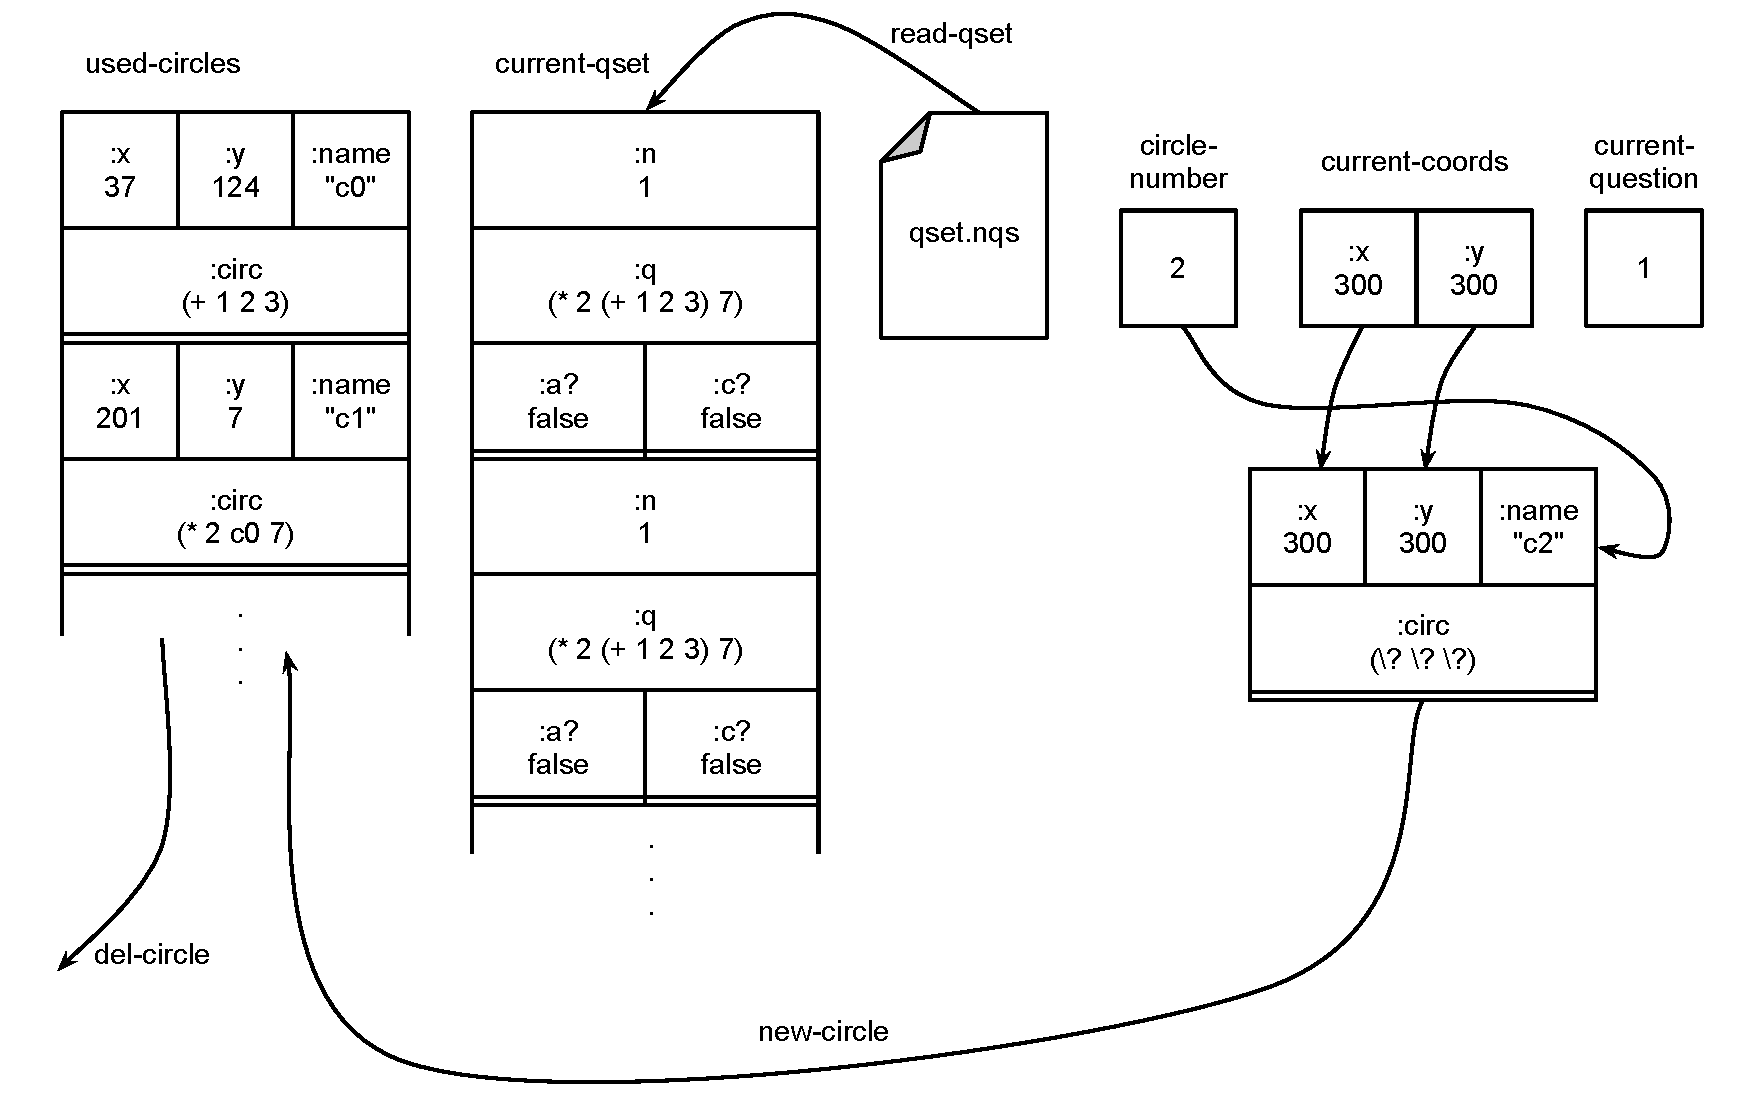
\includegraphics[width=\textwidth-2cm]{figs/nico_backend.pdf}
\end{center}
% \caption{A rough model of \emph{Nico's} management of mutable state.}
\caption{A model of \emph{Nico's} management of mutable state; the sixth agent is omitted as it is not utilised by the back-end.}
\end{figure}
\end{center}

\subsubsection{Circle Management}

\emph{Nico} includes two main functions for the management of circles: creation and deletion.  New circles are initialised to the following values:
% TODO: also maybe talk about kill-used-circles

\begin{center}
\begin{figure}[H]
\begin{center}
\begin{minipage}{2.5in}% {\textwidth-2cm}
\begin{Verbatim}[fontsize=\small,numbers=left]
{:x (- (:x @current-coords) 50)
 :y (- (:y @current-coords) 50)
 :name (str "c" @circle-number)
 :circ (\? \? \?)}
\end{Verbatim}
\end{minipage}
\end{center}
\caption{Circles are initialised on the current location of the mouse cursor, generating a name {\ttfamily "c}\emph{n}{\ttfamily "}, where \emph{n} is the number of circles that have previously been created, and with an initial expression of {\ttfamily (\textbackslash? \textbackslash? \textbackslash?)}.}
\end{figure}
\end{center}

This map is then stored in the list of circles.  The counter for the number of circles is incremented by one, and the user-facing canvas area is cleared and re-rendered.  This particular initial state for each circle was chosen so that the circle is centred upon the mouse cursor (rather than having its top-left corner appear at the location of the cursor if 50 had not been subtracted from the current co-ordinates), and so that its name is predictable, for use in other functions that refer to it; that is, the order in which the circles in the list were created can be inferred from their names if need be.  The circle is also initialised to a placeholder expression, rather than one of value 0, so that it does not interfere with the root-circle inference, which will be discussed later.

Deletion is a more complex function that removes a circle from the list.  It first compares its argument to the head of the circle list.  If it does not match its name or co-ordinate range (each circle is contained within an area of 100px$^2$), it recursively calls itself on the tail of the list, and appends the rejected circle to a new list.  If there is a match, it again calls itself on the tail of the main circle list, but does not add the head to the new list.  Thus, a list identical to the original list of circles is constructed, excluding only the matched circle.

This naïve implementation of deletion led to many problems: the function described above does not deal well with circles that are used as arguments to other circles.  When such a circle is removed from the main list, there still remain references to it in the circles that were using it as part of a larger calculation, causing the application to throw \verb¬java.lang.NullPointerException¬s.  As such, a `safe' version of circle deletion was implemented.  The safe deletion function works by first checking if any of the circle scurrently in the main list contain references to the circle being deleted.  If it is found that there are circles that contain references to it, the function determines if that circle is a root circle (see below), and, if so, uses the previous method of deletion to remove the circle and replace it with a similar circle that uses placeholder {\sfapp ?} values where there were references that would have been invalidated.  If the circle is non-root, the deletion function recursively calls itself upon the circle, thus removing all circles that formed the original chain dependent upon the circle to be deleted.  The circle can then safely be deleted using the previous method, and the intermediate circles are replaced.

This solved the problem of the leftover references to non-existant circles, but it has also given rise to a new problem: using this method, and in particular due to the stage in which the safe deletion function must call itself upon the other circles in the chain, deleting a circle that forms part of a chain deletes all of the links between the rest of the circles in the chain, from the circle being deleted down to the root circle.  On reflection, a better way to implement safe deletion would have been to include either as part of the rendering loop or as part of the safe deletion function a function to inspect the main circle list, checking for any invalid references and replacing them with \verb¬\?¬s, rather than doing it at delete-time.

\subsubsection{Evaluation}

There are two main stages required to evaluate the user's work: finding the root circle, into which all other circles feed, and evaluating a circle or collection of circles to give a valid, computable S-expression.

The root circle is the one circle in a finished diagram that is not used as an argument to any of the other circles.  Therefore, it can be found by searching through the list of circles, comparing each one to the rest of the list and discarding it if there are references to it in other circles.  As stated, in a {\bf finished} diagram, there can only be one root circle, so this method is sufficient for use in marking answers.  However, whilst the user is working, it is possible that they may construct two or more calculation structures in parllel, with intent to join them later.  In this case, there can be multiple root circles.  The method chosen to identify the root returns the first instance of a root circle that it comes across.  It would have been possible to, for example, add an extra {\sfapp Answer} panel for each root and maintain a total for each, but it was decided that this would be confusing for the user, who may not expect the structure of the application window to change.  This would also require a labelling system for circles and structures, which was abandoned in the user interface design as it is an unfamiliar concept to non-programmers and those without algebra: most of the target audience.

Once the root has been found, the user's diagram can then be evaluated to give an S-expression.  As each circle contains an S-expression for the calculation unit that it represents, all that needs to happen is for the references to other circles to be resolved, creating a nested S-expression that can simply have Clojure's \verb¬eval¬ called on it to return an answer.  This was, in fact, a significant reason for choose Clojure, as a dialect of LISP, as the language in which to program \emph{Nico}; as a homoiconic language, code to be evaluated later can easily be built up as a data structure, which can then be passed around, evaluated and otherwise utilised as is convenient.  By creating one unified S-expression representing the entire diagram, not only can the value of the structure be calculated, but other operations, such as the selective highlighting of the question (discussed below), can be performed.

\subsubsection{Question Management}

\emph{Nico} uses external files containing sets of questions to provide tasks for the user to complete.  An NQS (\emph{Nico} Question Set) file is simply a plain text file contaning S-expressions corresponding to questions, separated by newlines.  This particular approach was chosen so that questions can easily be read in using functionality provided by Clojure's standard library.  Nico is then able to navigate between questions by setting the agent containing the current question to the value of the desired question in the list.

A future extension to this project could be to develop a partner application to \emph{Nico} to aid tutors unfamiliar with LISP to develop their own question sets in a more `user-friendly' manner, rather than by transcribing lists of problems into S-expressions.

\subsection{Interaction Handler}
% the bit that handles all the application shit: render, main-window, etc.
% talk about jfx2 vs. guiftw/swt vs. seesaw/swing
% talk about main-window here i guess?
% talk about dialogue boxes
%
% \emph{{\sc Note:} These paragraphs aren't in the correct order yet; I've just been writing things that I want to include in this subsection, and will reorder them when I have a better idea of where this bit's going.}

The interaction handler is a collection of functions that form the `middle
layer' of the application: that is, the functions that arbitrate between the
back-end and the user interface.

The rendering function is called every time the mouse is moved, or when what is displayed on the canvas needs to be updated.  It paints a white rectangle over the canvas area, draws a bin icon in the corner (for circle, deletion, see information on the control scheme below) and iterates across the circle list, drawing a circle to match each element.  References to other circles are visualised as lines extending from the source circle to the appropriate argument slot on the recipient circle.  By re-rendering every time the mouse is moved, rather than continously, the application does not have to render when the canvas is not being changed, as every action in the control scheme requires some use of the mouse.

\subsubsection{GUI Libraries}

The original intention of the project was to develop \emph{Nico} using the JavaFX library.
However, a number of difficulties were encountered with this: firstly, JavaFX
version 2.0 was not available for Linux, the primary development environment, at
the time of beginning the project.  Installation was attempted on a
Windows machine, but caused a number of problems. In the interest of making progress, it was decided to proceed
using the Eclipse Foundation's SWT toolkit and Szymon Witamborski's
corresponding Clojure bindings, \emph{GUI FTW!} \cite{GuiFtw}.  During the development of the user interface, many problems were encountered with SWT and \emph{GUI FTW!}, particularly regarding drawing
arbitrary shapes on the canvas area and extracting user input from
dialogue boxes.  To keep the project on-schedule, the application was migrated to Java Swing,
using David Ray's \emph{Seesaw} library to provide bindings for
Clojure \cite{Seesaw}.

\subsubsection{Main Window}

At the heart of the interaction handler is the structure defining the main window, which comprises the majority of the user interface.  It controls what is to be displayed and the actions to be performed under certain conditions.  It listens for certain events (i.e. user input), and prompts the user for input when required.

Of particular note are the various listeners embedded into the main window structure that monitor the canvas for mouse-based events.  While the application is running, it listens for five mouse-based events: motion, dargging, a button press, a button release and a button click.\footnote{It should be noted that a mouse click is defined by Java as a button press followed by a button release, and that, upon a click, it issues a press event, followed by a release event, followed by a click event. \cite{JavaApi}}  When motion is detected, the canvas is cleared and re-rendered, as mentioned above.  Motion also triggers a check to determine whether or not the mouse is over a circle; if it is, a highlighting function is called.  This draws a ring around the circle currently being moused over, and also performs a string comparison:  using the same function written to convert the questions into traditional mathematics for display in the information panel, the circle's S-expression is converted and compared to the question string to see if it appears as a substring.  If so, the appropriate section of the question string is also highlighted, to help reinforce the notion of the circle notation as a metaphor for calculation.  It was decided to implement this a string search, rather than by using the actual S-expressions for the question and for the circle's calculation as although this would be a more efficient method to determine whether or not a circle corresponds to a part of the question, it is less efficient to do so and then calculate where the matched S-expression appears, rather than just matching a potential substring against a longer string.

\begin{center}
\begin{figure}[H]
\begin{center}
\subfloat[]{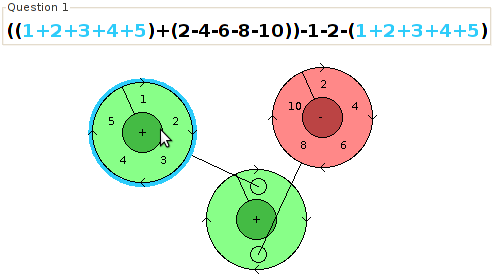
\includegraphics[height=\textwidth/3-1cm]{figs/nico_hi1.png}}
\subfloat[]{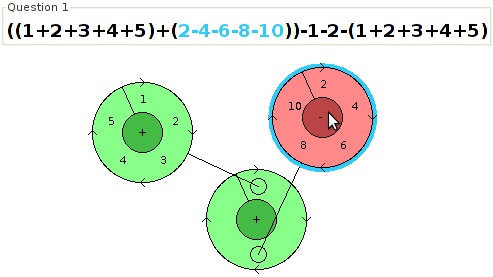
\includegraphics[height=\textwidth/3-1cm]{figs/nico_hi2.png}}
\\
\vspace{0.5cm}
\subfloat[]{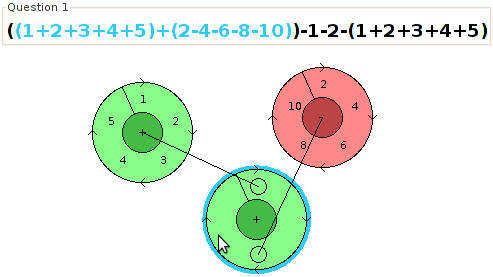
\includegraphics[height=\textwidth/3-1cm]{figs/nico_hi3.png}}
\end{center}
\caption{Three instances of the question text being highlighted as a corresponding circle is moused-over.}
\end{figure}
\end{center}

\subsubsection{Control Scheme}

Upon the detection of a mouse click, the software must determine the exact context in whcih the mouse was clicked, as this constitutes much of the application's control scheme.  The mouse's current co-ordinates on the canvas, as well as information regarding which mouse button was pressed and any modifiers that were active, are used to determine the correct action to take, as illustrated in \emph{Fig. x.y}.

\begin{center}
\begin{figure}[H]
\begin{center}
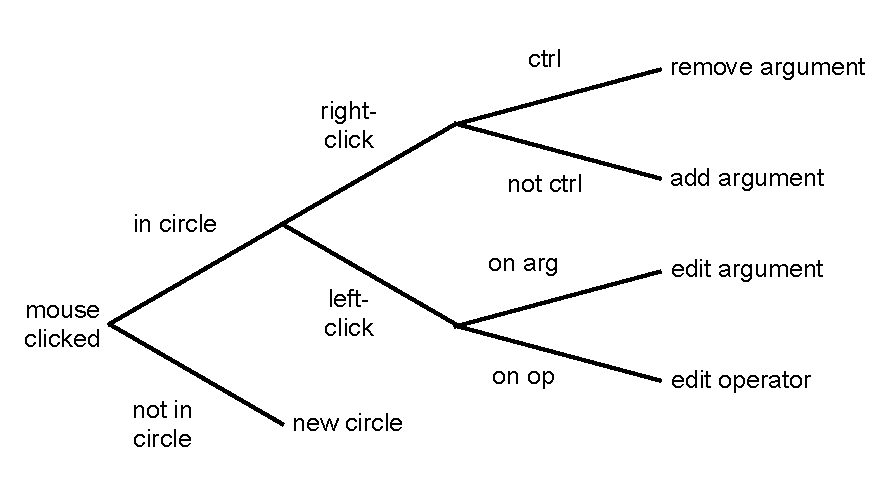
\includegraphics[width=\textwidth-4cm]{figs/nico_click.pdf}
\end{center}
\caption{Decision tree to determine the appropriate response to a mouse click event.}
\end{figure}
\end{center}

A more in-depth analysis of the control scheme follows.

\begin{itemize}
\item Mouse not in circle
\begin{itemize}
\item A blank circle is created, centred on the current location of the mouse cursor.  It has two arguments, {\sfapp ?} and {\sfapp ?}, and its operator is {\sfapp ?}.
\end{itemize}
\item Mouse in circle
\begin{itemize}
\item Left-click
\begin{itemize}
\item Mouse on argument
\begin{itemize}
\item A small blue circle is drawn around the argument and a dialogue box is launched, containing a spinner with which to set the new value of the selected argument.
\end{itemize}
\item Mouse on operator
\begin{itemize}
\item A small blue circle is drawn around the argument and a dialogue box is launched, containing four radio buttons corresponding to the four arithmetic operations, with which to set the new value of the operator.
\end{itemize}
\end{itemize}
\item Right-click
\begin{itemize}
\item Ctrl key pressed
\begin{itemize}
\item The final argument is removed from the circle, down to a minimum of two arguments.  An alert box warns the user if they try to remove arguments when there are only two remaining.
\end{itemize}
\item Ctrl key not pressed
\begin{itemize}
\item A placeholder argument is added to the circle, up to a maximum of eight arguments.  An alert box warns the user if they try to add more than the maximum number of arguments.
\end{itemize}
\end{itemize}
\end{itemize}
\end{itemize}

\emph{Nico} also includes some drag-and-drop functionality in its control scheme.  When the application detects that a mouse press has occurred, if the event was triggered whilst the mouse cursor was over a circle, that circle's map is stored, along with the current system time in milliseconds and the mouse button that was pressed, in one of the agents.  A drag event then uses the information stored in the agent to perform one of two operations upon the circle.  If the left mouse button is held whilst dragging, the circle's positioning information is updated to the current co-ordinates of the mouse cursor.  If the right mouse button is held whilst dragging, a line is drawn from the circle to the current location of the mouse cursor, indicating that two circles are to be joined.  When the mouse passes over the argument slot of another circle, that line is fixed, and the target circle is updated such that the argument now has the value of a reference to the source circle.  When the mouse is released, the information in the agent is removed.  The drag-and-drop functionality was implemented thus as a drag-and-drop action constitutes a press event, followed by a drag event, followed by a relase event.  By storing information about the circle being dragged in an agent upon detecting a mouse press, the function called when dragging is detected can use and modify this information easily, without encountering the problems of defining new variables at runtime, as mentioned in the discussion of the application back-end.  This does not impact upon other mouse events involving presses and releases (e.g. clicking), as the agent is reinitialised upon every mouse release, regardless of whether or not the drag-and-drop agent was being used.

% do i need to mention *all* the times clear-screen and render are called?  it's kind of implicit (to me anyway)...
%
% \emph{{\sc Note:} This is as far as I've got (about halfway by my reckoning).  }\verb¬texcount¬\emph{ tells me I've got about 5,800 words.}
% \subsection{User Interface}
% do we even need this section?  applciation below might cover it, and to be fair it isn't really part of the architecture - listeners and that should probs go in interaction handler above
%
\section{User Interface}%{Application}
% application in which the language is manipulated
% talk about how the app has changed, show screenshots
% talk about how the app becamse more minimalist, to focus on the language itself
% language as a main focus, with useful information n shit around it in the app
% colour-coding text (though consider colour-blindness with the red and green text)
% question highlighting - talk about troubles with it, but also merits of including it
% do we need this section?  shouldn't this be the ui bit in the prev. section?
% have lost the ui bit in favour of having this as a separate section
% target audience - children (year 5), but also applications in remedial adult learning (i.e. can't be too childish)
% hence must be appealing, clear, easy-to-read, not too verbose
% prototypes! take screenshots of old versions

The user interface comprises the parts of the application which are
user-facing; that is, they are that which the user directly interacts with.
The development of \emph{Nico}'s user interface was key to the success of the
overall project, being primarily an experiment in human-computer interaction.

\begin{center}
\begin{figure}[H]
\begin{center}
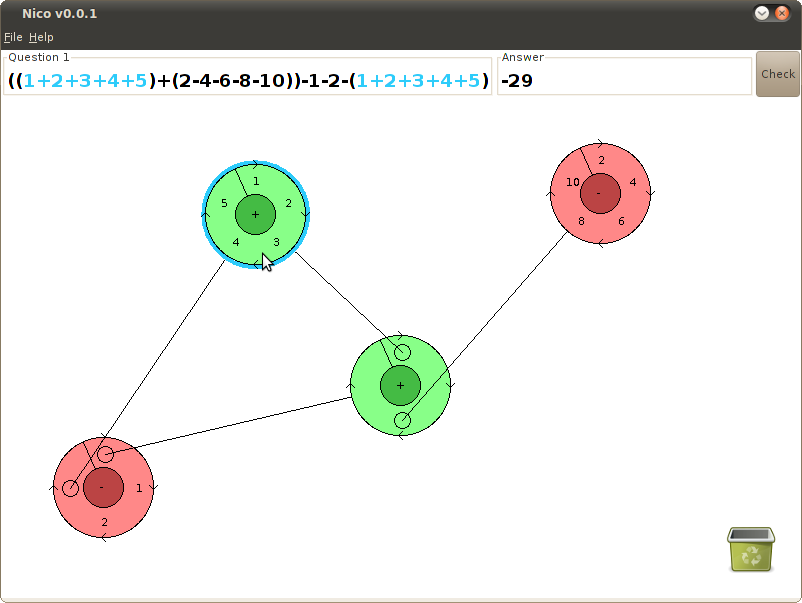
\includegraphics[width=\textwidth]{figs/nico_screen_01.png}
\end{center}
\caption{A screenshot of a \emph{Nico} session.}
\end{figure}
\end{center}

The application itself was kept fairly minimal: the aim was to emphasise the
notation as the most important aspect of the software.  As such, the main
application window, as shown above in \emph{Fig. x.y}, is mostly dedicated to
the canvas area in which the user answers the question.  The main application
window is split up into two main sections, the information panels that display the question being answered and the current
total of the user's calculation, as well as the {\sfapp Check} button to submit
the current total as the answer, and the large canvas
area in which the user is able to construct diagrams with which to answer the
question.

% TODO: diagram?  like the one in the notebook, showing the consequences of each possible action to illustrate the control scheme and notation

% why the '(\? \? \?) initial circle expr?
\emph{Nico} uses a predominantly mouse-based control system for the
construction of calculations in the application's notation.  Left-clicking on a
blank patch of canvas creates a new circle, initialised with two arguments,
{\sfapp ?} and {\sfapp ?}, and with operator {\sfapp ?} -- this approach was chosen, rather than providing the user with a null circle such as (0+0), to make it clear to the user that the new circle required attention, and so that it wouldn't interfere with the evaluation of the diagram; a new circle on its own could be found to be a root circle, leading to the possibility that the user's total could suddenly drop to 0, which would be confusing.  Right-clicking on a
circle increments its number of arguments by one, up to a maximum of eight.
Holding the Ctrl key and right-clicking on a circle decrements its number of
arguments by one, down to a minimum of two.  The user is warned by a popup if the exceed either of these boundaries.  The limit of two to eight arguments was decided upon as fewer than two arguments is an unfamiliar and not often useful concept from the perspective of the target audience.  Although Clojure is able to evaluate, for example, \verb¬(+ 1)¬ (returning \verb¬1¬), this is liable to lead to confusion on the part of the user.  The upper limit of eight arguments was set to prevent circles from becoming overcrowded and harder to read.
Circles can be moved around the
canvas by left-clicking and dragging the circle to the desired location.  If a
circle is dragged to the bin icon in the bottom left-hand corner of the screen,
then it is removed.  Originally, deletion was mapped to a mouse control, but in the interest of a simpler control scheme and with a limited number of mouse buttons, it was decided that an icon should be used instead.  This also has the advantage of demonstrating to the new user that work can be easily undone, encouraging exploration.  Left-clicking on a circle's operator brings up a dialogue
box with a selection of operators in it, with a radio button for each (see
\emph{Fig. x.y}).  Similarly, left-clicking on a circle's argument brings up a
dialogue box containing a spinner, which can be used to set a new value for
that argument, between -10 and 10.  The spinner is limited to this particular
range as this prevents the user from effectively using the software as a simple
calculator.  The limited range of numbers available means that the user must
still consider strategies such as partitioning or long multiplication,
focussing on how to solve the problem, rather than simply transcribing the
question into one circle that will complete the calculation for them.  The user is not required to calculate manually expressions using such small numbers, as it is assumed that the target audience are familiar with simple arithmetic.  To use
one circle as an argument to another, right-clicking and dragging allows the
user to drag a line ending in a circle to the desired slot on the recipient
circle.

\begin{center}
\begin{figure}[H]
\begin{center}
\subfloat[Editing a circle's operator]{
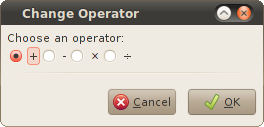
\includegraphics[width=\textwidth/2-2cm]{figs/nico_op.png}
}
\subfloat[Editing a circle's argument]{
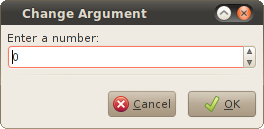
\includegraphics[width=\textwidth/2-2cm]{figs/nico_arg.png}
}
\end{center}
\caption{The dialogue boxes used to modify existing circles in the application.}
\end{figure}
\end{center}

% talk about colour-blindness
% why this colour scheme? psychological reasons?
% why not random or connection-based colours?
\emph{Nico} also uses colour-coding in various areas of the application, to
draw attention to important elements of the application.  Colour-coding has
been shown to faciliate more effective learning.  Indeed, Lamberski and Dwyer
note that
\begin{center}
\parbox[c]{\textwidth-2cm}{
\small
``[...] younger learners, for whom color in passive materials has been found to facilitate performance in less complex concept attainment tasks because of color's attention of motivation elements.  However, when younger learners have been given self-paced instructional materials containing color-coded reading and phonic concepts, similar positive results have been attained.'' \cite{Lamberski1983}
}
\end{center}
Circles are coloured according to their operators, clearly separating different
kinds of operations and making the notation more readable.  An alternative
method of colour-coding by the level of nesting was considered, but rejected on
the grounds that it could become confusing if a circle were reused (see
\emph{Fig. x.y}).

\begin{center}
\begin{figure}[H]
\begin{center}
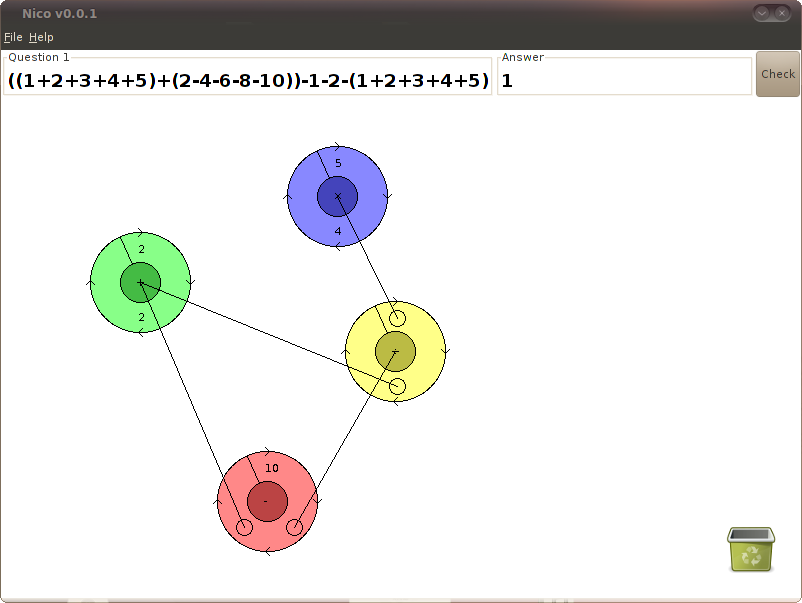
\includegraphics[width=\textwidth-2cm]{figs/nico_screen_02.png}
\end{center}
\caption{An example of where nesting-based colour-coding would be confusing.  The circle containing (2+2) can be considered to be both one and two circles removed from the root circle.}
\end{figure}
\end{center}

Colour-coding is also used in the information panels: positioning the mouse cursor over a circle highlights the part of
the question that it is likely to represent in blue, and also highlights the
circle with a blue outline.  When an answer is submitted, the text in the
answer panel turns red if the answer was incorrect, or green if the answer was
correct, providing an unintrusive form of feedback, allowing the user to
continue uninterrupted (i.e. no input is required) if their answer is wrong.

\begin{center}
\begin{figure}[H]
\begin{center}
\subfloat[Red text indicates that the answer submitted was incorrect]{
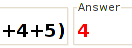
\includegraphics[width=\textwidth/3]{figs/nico_wrong.png}
}\hspace{2cm}
\subfloat[Green text indicates a correct answer; a dialogue box allows the user to progress to the next question when they are ready]{
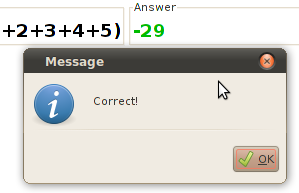
\includegraphics[width=\textwidth/3]{figs/nico_right.png}
}\\
\subfloat[The circle's operator is highlighted when it is being edited]{
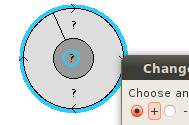
\includegraphics[width=\textwidth/3]{figs/nico_op_hi.png}
}\hspace{2cm}
\subfloat[An argument is highlighted when it is being edited]{
\includegraphics[width=\textwidth/3]{figs/nico_arg_hi.png}
}
\end{center}
\caption{Examples of colour-coding in \emph{Nico}.}
\end{figure}
\end{center}

During its development, \emph{Nico}'s user interface went through a number of
revisions.  Details of how the UI design developed over time follow.

\subsubsection{First Revision}
Initially, the application was intended to use more buttons (see
the prototype in \emph{Fig. x.y}, above), having more controls immediately
visible to the user.  In the first usable version of the interface, there were
a number of buttons that appeared down the side of the application.  Each
button ({\sfapp New}, {\sfapp Edit}, {\sfapp Delete}, etc.) would cause a
dialogue box to appear to the user, which required a circle to be specified by
name (at this point in the development of the project, it was required that the
user name each of their circles) before any operations could be performed upon
it.  The operations themselves were specified by typing the circle's name into a text field, followed, in the case of the creation and editing of circles, an S-expression specifying the mathematical expression that the circle was to represent.  Circles were all the same colour, and the text-highlighting and colour-coding operations had not yet been implmented.  It was also the case that the links between circles did not end in argument slots, but rather fed into the centre of the target circle.  This design was abandoned as the separation between the user and the diagram itself was too great; creating circles by specifying options in many only slightly different dialogue boxes and watching the results appear on the canvas did not feel like a natural way to interact with one's calculation, and hence would have been inappropriate for the target audience.  Indeed, forcing the user to commit to a design before even seeing it entailed much \emph{premature commitment}.  Requiring the user to use LISP S-expression syntax was also far from ideal, as the user then had to learn this syntax in order to use the program.  The intention of the project is not to require the user to spent a significant amount of time learning how to use the system before it becomes a useful tool to them.  Quite apart from this, a user familiar with LISP is also unlikely to need the aid of the circle metaphor to visualise expressions.
% how did we know the separation was too great?
% avoid "similar-but-slightly-different"

\subsubsection{Later Revisions}
Later revisions of the software removed the buttons and implemented a system of
context menus with which to construct answers. Right-clicking on a blank patch
of the canvas gave the user the option to create a new circle, and right-
clicking on an existing circle presented the user with the option to either
edit or delete that circle.  Choosing to either create of edit a circle
displayed a dialogue box (\emph{Fig. x.y}), with many options for the user to
choose from: the name and operator of a circle could be set, with up to eight
arguments could be enabled, with a choice of either a number (set by a slider)
or another circle (chosen using a list of radio buttons that was generated upon
opening the dialogue box) as the value of that argument.  Answer-checking was
also made automatic: as soon as the total reaches a value equal to that of the
answer to the question, the user is immediately told so, and moved on to the
next question.  The circles at this point were still one colour only, and there
was no expression-highlighting.  The colour-coded totals had been implemented by
this point.  This design was ultimately abandoned as, again, it separated the
user from their own work too much.  Although this design was an improvement,
allowing the user to interact directly with the canvas to perform operations
upon circles that were able to specified by pointing with the mouse, rather
than by typing out a name, the grand unified dialogue box still required the
user to perform operations without it being entirely obvious what the
consequences would be, thus requiring an unnecessary amount of
\emph{premature commitment} from the user.  In addition to this, the act of
visualising the circle to be created whilst setting the many options available
in the dialogue box constituted an unnecessary \emph{hard mental operation}.
The automatic answer-checking was also a problem, as it did not give the user a
chance to review their answer before proceeding.  Indeed, it did not give the
user a chance to learn from their mistakes, say for example if they had
accidentally reached the right answer as part of a larger, incorrect
calculation that they had previously intended to make.

\subsubsection{Current Revision}
The final, current revision of the software reintroduces the {\sfapp Check}
button to address the issues with the automatic answer-checking in the
previous version of the application.  It also introduces the control scheme
detailed above, allowing the user to feel more like they are directly
manipulating their work in progress, with each action having clear
consequences.  A colour scheme for the circles was implemented, to make the
notation easier to read, and the expression-highlighting functionality was also
introduced, along with the other means of highlighting, as shown above.
Finally, the bin icon was introduced after deciding that a control for deletion
was not an ideal approach, as detailed above.

\begin{center}
\begin{figure}[H]
\begin{center}
{\Huge \sfapp OLD VERSIONS OF THE APP LOL}
\end{center}
\caption{\emph{Nico}'s user interface went through a number of revisions before reaching its current state.}
\end{figure}
\end{center}

\subsection{Notation}%metaphor?
% graphical language itself
% show previous versions
% talk about how the circles have to make clear e.g. arg order
% talk about how circles had to be improved, show iterations
% more screens: old versions of the language to compare

\begin{center}
\begin{figure}[H]
\begin{center}
{\Huge \sfapp OLD VERSIONS OF THE NOTATION LOL}
\end{center}
\caption{The notation used also went through a number of revisions before reaching its current state.}
\end{figure}
\end{center}

The notation itself was also revised several times during the development of
the application.  The original vision of the notation can be seen in
\emph{Fig. x.y}.  The first implementation of the notation consisted of
uniformly-coloured circles connected by lines feeding into the centre of the
recipient circle.  There were no placeholder values; these were unnecessary as
the system of dialogue boxes meant that at no point could a circle have any
aspect of itself in an undefined state.  There was also no indication of
argument ordering, which is acceptable when the operator is commutative (i.e.
addition or multiplication), but for operations where this is not the case,
this can quickly become confusing.  Although the ordering and placement of
arguments was defined, with no indication of this, the user is required to
figure this out through experience, which is counter to the intentions of the
software.  As mentioned above, it should not be required that the user spend a
significant amount of time learning how to use the system, especially due to
deficiencies in the notation.  Another, greater, problem related to argument
ordering was that of the circles that linked to other circles.  With all input
circles pointing to the operator at the centre of their target circle, it was
not at all clear in which order the input circles evaluated, neither relative
to each other nor to the other arguments in the circle.

% TODO: poss. a figure showing close-ups/details of newest notation?

The notation changed somewhat to address the problems listed above.  In its
current revision, the notation has had a number of features added.  Firstly,
the circles are now colour-coded by operator, making it easier for the user to
distinguish between different kinds of circles.  The circles themselves have
also been embellished slightly with the addition of a line denoting the star of
the expression, just to the side of the first argument at the top of the
circle.  Smalls arrow have also been added to the edge of the circles to
indicate in which direction the arguments should be read.  Finally, the links
between circles have been changed such that they now occupy an argument slot
that could otherwise be taken by a number, with a circle on the end of the link
line to clearly show where the link terminates.
% TODO: more cogdims!  ALWAYS more cogdims!

% TODO: testing?  or does that go in the next chapter?

\section{Summary}

In this chapter, the implementation of the project was discussed in some
detail, as well as the challenges that were faced during this development
phase.  The software itself fulfils and exceeds the criteria for success
outlined in the project proposal, being a complete and usable system that
improves greatly, in terms of cognitive dimensions, upon the traditional method
of handwritten arithmetic.  Third-party libraries, in particular Seesaw, were
used where appropriate.  The application divides into three main sections: the
back-end, handling mathematical operations and memory management, the
interaction handler, helping the user interface to interface with the back-end,
and the user interface itself.  The user interface was revised many times to
correct deficiencies in the design that would have led to a poor user
experience, and the back-end and interaction handler were also both restructured
as new demands upon the software became apparent.

In the next chapter, the software will be evaluated, discussing test results
and the user study that was conducted as an extension to the project.

\cleardoublepage
\chapter{Evaluation}

This chapter concerns the testing and evaluation of \emph{Nico}; carried out to determine the quality and utility of the software.

\section{Testing}% {Defect Management and Testing}% {Backend Testing}
% used slime/swank with test lines as comments to be evaluated with C-x C-e
% emacs/slime/swank as ide; ideal for lisps!
% lein test framework - need to actually set up some tests first though!
% clojure test-is; see http://en.wikibooks.org/wiki/Clojure_Programming/Tutorials_and_Tips#Unit_Testing_in_Clojure

% does C-x C-e *actually* count as unit testing?  i mean, i *did* test small bits and then test bigger bits after i'd established that the smaller bits worked...
% apparently it does! w00t
% also talk about integration testing (after the units have been tested, testing the bits that use those units), and see the link in alistair's email re other levels of testing
Throughout the development of the software, I performed unit tests to ensure
the integrity of my code.  My development environment of choice, GNU Emacs
using SLIME/SWANK and clojure-mode, includes functionality such that
commented-out lines of code can be evaluated at will.  As such, it was possible
for me to write unit tests into the main body of my code, evaluating them
whenever a change may have affected how a function behaved.  In the interests
of tidiness and code readability, many tests were removed as they became
unnecessary later on in the devlopment in the project, but \emph{Fig. x.y}
shows one of the test blocks that were left in the most recent revision of the
source code.

\begin{center}
\begin{figure}[H]
\begin{center}
\begin{minipage}{11.7cm}% {\textwidth-2cm}
\begin{Verbatim}[fontsize=\tiny,numbers=left]
(defn detect-subs
  "Returns a list of maps containing start and end indices showing where a substring c appears in the superstring q."
  [c q]
  (loop [s (cond (= (subs q
                          (- (count q) (count c))
                          (count q)) c) (split q
                                               (re-pattern
                                                (escape
                                                 c
                                                 {\+ "\\+"
                                                  \( "\\("
                                                  \) "\\)"})))
                 :else (butlast (split q
                         (re-pattern
                          (escape
                           c
                           {\+ "\\+"
                            \( "\\("
                            \) "\\)"})))))
         i 0
         l '()]
    (cond (empty? s) (reverse l)
          (= c (subs q
                     (+ i (count (first s)))
                     (+ i (count (first s)) (count c)))) (recur (rest s)
                                                                (inc i)
                                                                (cons {:s (+ i (count (first s)))
                                                                       :e (+ i (count (first s)) (count c))}
                                                                      l))
          :else (recur s (inc i) l))))

;; (def tq (lisp-to-maths (eval (:q (first @current-qset)))))
;; (subs tq (:s (nth (detect-subs "1+2" tq) 0)) (:e (nth (detect-subs "1+2" tq) 0)))
;; (subs tq (:s (nth (detect-subs "1+2" tq) 1)) (:e (nth (detect-subs "1+2" tq) 1)))
;; (subs tq (:s (nth (detect-subs "1+2" tq) 2)) (:e (nth (detect-subs "1+2" tq) 2)))
;; (let [s "roflolmaomglolwtf" i (detect-subs "lol" s)] (subs s (:s (nth i 0)) (:e (nth i 0))))
;; (let [s "roflolmaomglolwtf" i (detect-subs "lol" s)] (subs s (:s (nth i 1)) (:e (nth i 1))))
;; (let [s "roflolmaomglolwtf" i (detect-subs "lol" s)] (subs s (:s (nth i 2)) (:e (nth i 2))))

;; (let [s "0123456789" i (detect-subs "456" s)] (subs s (:s (first i)) (:e (first i))))
;; (let [s "roflolmaomglolwtf" i (detect-subs "lol" s)] (subs s (:s (first i)) (:e (first i))))
;; (let [s "fagaha" i (detect-subs "a" s)] (subs s (:s (first i)) (:e (first i))))
;; (let [s "lalala" i (detect-subs "a" s)] (subs s (:s (first i)) (:e (first i))))
;; (detect-subs (lisp-to-maths (eval-circle (find-circle "c0"))) (lisp-to-maths (eval (:q (first @current-qset)))))
;; (let [s "dcbabcd" i (detect-subs "a" s)] (subs s (:s (first i)) (:e (first i))))
;; (let [s "dcbabcd" i (detect-subs "a" s)] (subs s (:s (nth i 1)) (:e (nth i 1))))

\end{Verbatim}
\end{minipage}
\end{center}
\caption{An example of a block of inline tests, taken from {\ttfamily core.clj}, showing some tests to be run to test the implementation of {\ttfamily detect-subs}.}
\end{figure}
\end{center}


\section{UI Evaluation}
% user testing
% graphs

\subsection{Notation Evaluation}
% user testing
% graphs

\section{User Study}
% results
% pilot study - ellie suggested switching left/right-clicks in control scheme, implemented before main study

To assess the utility of the software relative to handwritten arithmetic, a
user study was conducted, allowing real users to get to grips with the system,
and provide feedback on it.  To this end, users were given a tutorial video and
a questionnaire (see \emph{Appendix A} for the full questionnaire) to complete
whilst using the software.

Originally, it was the intention of this project to perform a user study upon
a `test class' of Year 5 pupils at an actual school, but the ethical
complications involved with working with vulnerable individuals were so great
as to make such a study impractical, given the time constraints of this
dissertation; in addition to obtaining the approval of the Ethics Committee and
the permission of a school to conduct the study, consent forms would have to be
distributed to the test class, taken home, signed by the pupils' guardians,
returned to the school and returned to myself.  It was, therefore, decided that
the software should be tested upon a group of students not currently reading a
`mathematical' subject, such as the Natural Sciences Tripos, the Mathematical
Tripos or the Computer Science Tripos, which necessitate a high level of
mathematical aptitude and experience.

Test subjects were first asked to sign a statement of informed consent, giving
their consent to participate in the study, and were then asked if they had
previously used \emph{Nico}, and to indicate their confidence in their ability
to solve simple mathematical problems on a five-point Likert item.  Users were
then divided into two groups.  The first watched the tutorial video and were
allowed to explore the application in a `sandbox' environment for five
minutes.  They then completed one question set using \emph{Nico}, and answered
the same questions by hand.  The second group completed the questions by hand
before watching the video and using the software.  The time taken to answer
each question was recorded, with \emph{Nico} including functionality to query
the system time as the user progressed and the handwritten questions being
timed using a stopwatch.  Both groups were then asked to complete a series of
questions to provide feedback on the software, taking questions from Blackwell
and Green's sample questionnaire. \cite{Blackwell2000}

\subsection{Pilot Study}
% changes, improvements

A pilot study was conducted with one test subject, to assess the feasibility of
the experiment that had been designed.  The outcome of this study was to make
changes to several areas of the test, and a small change to the control scheme
of the application itself.  Firstly, the pilot test subject noted that the
original version of the tutorial video for \emph{Nico} was hard to follow; it
used subtitles to convey information, which the test subject felt were hard to
read and understand in the time given.  The subject also noted that some of the
questions in the feedback section were confusing or seemingly irrelevant to
this particular application, and was unsure of how to answer them.  The final
piece of feedback that the subject provided was that the control scheme of the
application seemed counterintuitively focussed upon the right mouse button,
where it would have felt more natural to the user to have used the left.

In the interests of improving the study, I acted upon the subject's advice.
The video was reproduced using a voiceover rather than subtitles, making it
easier to follow.  Some of the less relevant questions were removed from the
feedback section, leaving those more applicable to \emph{Nico}.  Finally, the
control scheme was revised, assigning the left mouse button to primary
functions such as the creation and editing of circles, and the right to
functions such as changing the number of arguments.

\subsection{Results}
% data, graphs, analyses
% p-values:
% q1:  t = -8.0204, df = 7, p-value = 8.968e-05 <- sig
% q2:  t = -8.0493, df = 7, p-value = 8.764e-05 <- sig
% q3:  t = -8.9296, df = 7, p-value = 4.489e-05 <- sig
% q4:  t = -2.9592, df = 7, p-value = 0.02113   <- sig
% q5:  t = -5.288, df = 7, p-value = 0.001138   <- sig
% q6:  t = -1.3149, df = 7, p-value = 0.2300
% q7:  t = 2.3688, df = 7, p-value = 0.0497     <- sig
% q8:  t = 3.1, df = 7, p-value = 0.01732       <- sig
% q9:  t = 4.0293, df = 7, p-value = 0.005      <- sig
% q10: t = 2.1298, df = 7, p-value = 0.0707

The results of the tests are shown in \emph{Table x.y}, listing the times taken
for each subject to answer the questions both by hand and using \emph{Nico}.

\begin{center}
\begin{table}[H]
\begin{center}
\begin{tabular}{|r||r|r||r|r||r|r||r|r|}
\cline{2-9}
\multicolumn{1}{c|}{} & \multicolumn{8}{c|}{Group 1}\\ \cline{2-9}
\multicolumn{1}{c|}{} & \multicolumn{2}{c||}{Subject 1} & \multicolumn{2}{c||}{Subject 2} & \multicolumn{2}{c||}{Subject 3} & \multicolumn{2}{c|}{Subject 4}\\ \hline
\multicolumn{1}{|c||}{Question} & \multicolumn{1}{c|}{Hand} & \multicolumn{1}{c||}{\emph{Nico}} & \multicolumn{1}{c|}{Hand} & \multicolumn{1}{c||}{\emph{Nico}} & \multicolumn{1}{c|}{Hand} & \multicolumn{1}{c||}{\emph{Nico}} & \multicolumn{1}{c|}{Hand} & \multicolumn{1}{c|}{\emph{Nico}}\\ \hline \hline
Q1 & 4600 & 19547 & 3100 & 34094 & 1800 & 24657 & 1300 & 38891\\ \hline
Q2 & 8800 & 23313 & 7000 & 24329 & 6300 & 17437 & 5400 & 12031\\ \hline
Q3 & 20600 & 53500 & 13600 & 36360 & 10100 & 40798 & 10700 & 31813\\ \hline
Q4 & 36200 & 54375 & 26400 & 60156 & 14200 & 79704 & 23800 & 50094\\ \hline
Q5 & 61900 & 103344 & 39600 & 79844 & 26500 & 103221 & 33400 & 61064\\ \hline
Q6 & 213400 & 224406 & 190300 & 215376 & 84900 & 172940 & 181700 & 154691\\ \hline
Q7 & 235200 & 165813 & 1996000 & 103376 & 909000 & 48922 & 194200 & 52595\\ \hline
Q8 & 259500 & 306625 & 282500 & 158094 & 147200 & 138581 & 256700 & 155347\\ \hline
Q9 & 304400 & 230953 & 313500 & 123626 & 159800 & 183722 & 271700 & 196144\\ \hline
Q10 & 416500 & 307734 & 357700 & 213642 & 197100 & 245161 & 322200 & 235364\\ \hline
\multicolumn{9}{c}{}\\ \cline{2-9}
\multicolumn{1}{c|}{} & \multicolumn{8}{c|}{Group 2}\\ \cline{2-9}
\multicolumn{1}{c|}{} & \multicolumn{2}{c||}{Subject 1} & \multicolumn{2}{c||}{Subject 2} & \multicolumn{2}{c||}{Subject 3} & \multicolumn{2}{c|}{Subject 4}\\ \hline
\multicolumn{1}{|c||}{Question} & \multicolumn{1}{c|}{Hand} & \multicolumn{1}{c||}{\emph{Nico}} & \multicolumn{1}{c|}{Hand} & \multicolumn{1}{c||}{\emph{Nico}} & \multicolumn{1}{c|}{Hand} & \multicolumn{1}{c||}{\emph{Nico}} & \multicolumn{1}{c|}{Hand} & \multicolumn{1}{c|}{\emph{Nico}}\\ \hline \hline
Q1 & 1200 & 22299 & 2100 & 23516 & 2600 & 16142 & 2600 & 21985\\ \hline
Q2 & 2200 & 24530 & 5600 & 19015 & 7200 & 16875 & 7200 & 23422\\ \hline
Q3 & 17300 & 47620 & 7600 & 29735 & 18400 & 27923 & 15900 & 48470\\ \hline
Q4 & 23000 & 50704 & 20700 & 43094 & 25300 & 37516 & 38600 & 174160\\ \hline
Q5 & 46600 & 134828 & 33300 & 70313 & 35500 & 58954 & 72400 & 98846\\ \hline
Q6 & 199900 & 629835 & 136400 & 164891 & 99000 & 113659 & 266600 & 252708\\ \hline
Q7 & 202400 & 80277 & 142200 & 48890 & 1106000 & 52954 & 272900 & 72767\\ \hline
Q8 & 295900 & 248736 & 182000 & 107375 & 184700 & 78001 & 348900 & 257224\\ \hline
Q9 & 312900 & 152185 & 204100 & 118594 & 200500 & 67485 & 384500 & 144753\\ \hline
Q10 & 357300 & 238300 & 261600 & 203110 & 237500 & 324581 & 472900 & 270177\\
\hline
\end{tabular}
\end{center}
\caption{Table showing the time in milliseconds taken by each test subject to complete each question, by hand and using the software.}
\end{table}
\end{center}

This data can be visualised using a series of plots, as follows.

\begin{center}
\begin{figure}[H]
\begin{center}
\includegraphics[width=\textwidth-2cm]{figs/graphs/q1.png}
\end{center}
\caption{Time taken in milliseconds per subject to answer Question 1.}
\end{figure}
\end{center}

\begin{center}
\begin{figure}[H]
\begin{center}
\includegraphics[width=\textwidth-2cm]{figs/graphs/q2.png}
\end{center}
\caption{Time taken in milliseconds per subject to answer Question 2.}
\end{figure}
\end{center}

\begin{center}
\begin{figure}[H]
\begin{center}
\includegraphics[width=\textwidth-2cm]{figs/graphs/q3.png}
\end{center}
\caption{Time taken in milliseconds per subject to answer Question 3.}
\end{figure}
\end{center}

\begin{center}
\begin{figure}[H]
\begin{center}
\includegraphics[width=\textwidth-2cm]{figs/graphs/q4.png}
\end{center}
\caption{Time taken in milliseconds per subject to answer Question 4.}
\end{figure}
\end{center}

\begin{center}
\begin{figure}[H]
\begin{center}
\includegraphics[width=\textwidth-2cm]{figs/graphs/q5.png}
\end{center}
\caption{Time taken in milliseconds per subject to answer Question 5.}
\end{figure}
\end{center}

\begin{center}
\begin{figure}[H]
\begin{center}
\includegraphics[width=\textwidth-2cm]{figs/graphs/q6.png}
\end{center}
\caption{Time taken in milliseconds per subject to answer Question 6.}
\end{figure}
\end{center}

\begin{center}
\begin{figure}[H]
\begin{center}
\includegraphics[width=\textwidth-2cm]{figs/graphs/q7.png}
\end{center}
\caption{Time taken in milliseconds per subject to answer Question 7.}
\end{figure}
\end{center}

\begin{center}
\begin{figure}[H]
\begin{center}
\includegraphics[width=\textwidth-2cm]{figs/graphs/q8.png}
\end{center}
\caption{Time taken in milliseconds per subject to answer Question 8.}
\end{figure}
\end{center}

\begin{center}
\begin{figure}[H]
\begin{center}
\includegraphics[width=\textwidth-2cm]{figs/graphs/q9.png}
\end{center}
\caption{Time taken in milliseconds per subject to answer Question 9.}
\end{figure}
\end{center}

\begin{center}
\begin{figure}[H]
\begin{center}
\includegraphics[width=\textwidth-2cm]{figs/graphs/q10.png}
\end{center}
\caption{Time taken in milliseconds per subject to answer Question 10.}
\end{figure}
\end{center}

A two-sample, paired \emph{t}-test using an \emph{α} value of 0.05 was used to
determine whether or not the difference between the mean time taken to answer
each question by hand and using \emph{Nico} was statistically-significant.  The
paired \emph{t}-test was chosen as the samples are not independent.  The
results of the \emph{t}-tests on each question's datasets are shown in
\emph{Table x.y}.  The data is assumed to fit a normal distribution.  A
Shapiro-Wilk test was considered to test each dataset for normality, but the
sample size of eight data points per set (i.e. eight subjects for each
question) was deemed to be too small for such a test to have meaningful results.

% remove df (degrees of freedom)?
\begin{center}
\begin{table}[H]
\begin{center}
\begin{tabular}{|r|r|r|r|r|}
\hline
Question & \emph{t} & \emph{df} & \emph{p} & Significant?\\ \hline \hline
Q1 & -8.0204 & 7 & 0.00008968 & Yes\\ \hline
Q2 & -8.0493 & 7 & 0.00008764 & Yes\\ \hline
Q3 & -8.9296 & 7 & 0.00004489 & Yes\\ \hline
Q4 & -2.9592 & 7 & 0.02113 & Yes\\ \hline
Q5 & -5.288 & 7 &  0.001138 & Yes\\ \hline
Q6 & -1.3149 & 7 & 0.2300 & No\\ \hline
Q7 & 2.3688 & 7 &  0.0497 & Yes\\ \hline
Q8 & 3.1 & 7 & 0.01732 & Yes\\ \hline
Q9 & 4.0293 & 7 & 0.005 & Yes\\ \hline
Q10 & 2.1298 & 7 & 0.0707 & No\\
\hline
\end{tabular}
\end{center}
\caption{Table showing the results of the paired \emph{t}-test comparing the distribution of times taken to answer each question by hand and using the software, using an \emph{α} value of 0.05.}
\end{table}
\end{center}

As the \emph{p}-values in the above table indicate, there was a significant
difference in performance between using \emph{Nico} and completing the
questions by hand.  For the first five questions, the time taken to complete
the questions is markedly increased by using the software.  This is somewhat to
be expected;  the first five questions were `warm-up' questions, requiring a
maximum of three separate calculations to solve and with all numbers involved
in each calculation being less than ten.  Such questions were included to give
the user a chance to get used to solving simple problems using \emph{Nico},
before moving on to more complex tasks.  By the sixth question, there is no
longer a statistically-significant difference between using the software and
completing the questions by hand.  This particular question still uses numbers
less than ten, but requires several more nested calculations to solve,
suggesting that \emph{Nico} offers some improvement where the handwritten
method is lacking, but also that this is offset by the greater time required to
input very simple expressions into the application.  The final four questions
introduced numbers greater than ten, include many subcalculations and large
numbers.  For the seventh, eighth and ninth questions, \emph{Nico} offers a
statistically-significant improvement.  These questions involve the
manipulation of larger numbers, requiring strategies that go beyond simply
recalling number bonds, such as partitioning or long multiplication.  It is
these types of questions that \emph{Nico} is intended to make easier for the
user, and the often-dramatic decrease in the time taken to solve such questions
is shown to great effect here.  The tenth question, on reflection, was not
well-chosen.  It is comparable in difficulty to the fifth question, being a
series of simple subcalculations with numbers less than ten.  Though there are
more calculations to perform, and one operation involving a large number at the
end,  this question is not especially challenging to solve by hand, and as such
the lack of a significant difference between using the software and not doing
so is not entirely unexpected.  The simple subcalculations are easier to
perform by hand, and combining them is faster using \emph{Nico}.

Data were also collected regarding how well the questions were answered by each
user, which follow.

\begin{center}
\begin{table}[H]
\begin{center}
\begin{tabular}{|r||r|r||r|r||r|r||r|r|}
\cline{2-9}
\multicolumn{1}{c|}{} & \multicolumn{8}{c|}{Group 1}\\ \cline{2-9}
\multicolumn{1}{c|}{} & \multicolumn{2}{c||}{Subject 1} & \multicolumn{2}{c||}{Subject 2} & \multicolumn{2}{c||}{Subject 3} & \multicolumn{2}{c|}{Subject 4}\\ \hline
\multicolumn{1}{|c||}{Question} & \multicolumn{1}{c|}{Marks} & \multicolumn{1}{c||}{Errors} & \multicolumn{1}{c|}{Marks} & \multicolumn{1}{c||}{Errors} & \multicolumn{1}{c|}{Marks} & \multicolumn{1}{c||}{Errors} & \multicolumn{1}{c|}{Marks} & \multicolumn{1}{c|}{Errors}\\ \hline \hline
Q1 & 1 & 0 & 1 & 0 & 1 & 0 & 1 & 0\\ \hline
Q2 & 1 & 0 & 1 & 0 & 1 & 0 & 1 & 0\\ \hline
Q3 & 1 & 0 & 1 & 0 & 1 & 0 & 0 & 0\\ \hline
Q4 & 1 & 0 & 1 & 0 & 1 & 0 & 1 & 0\\ \hline
Q5 & 1 & 0 & 1 & 0 & 1 & 0 & 1 & 0\\ \hline
Q6 & 0 & 0 & 0 & 0 & 0 & 0 & 0 & 0\\ \hline
Q7 & 1 & 0 & 1 & 0 & 1 & 0 & 1 & 0\\ \hline
Q8 & 0 & 0 & 1 & 1 & 1 & 0 & 1 & 0\\ \hline
Q9 & 0 & 0 & 1 & 0 & 1 & 1 & 1 & 1\\ \hline
Q10 & 1 & 0 & 0 & 0 & 1 & 0 & 1 & 0\\ \hline
\multicolumn{9}{c}{}\\ \cline{2-9}
\multicolumn{1}{c|}{} & \multicolumn{8}{c|}{Group 2}\\ \cline{2-9}
\multicolumn{1}{c|}{} & \multicolumn{2}{c||}{Subject 1} & \multicolumn{2}{c||}{Subject 2} & \multicolumn{2}{c||}{Subject 3} & \multicolumn{2}{c|}{Subject 4}\\ \hline
\multicolumn{1}{|c||}{Question} & \multicolumn{1}{c|}{Marks} & \multicolumn{1}{c||}{Errors} & \multicolumn{1}{c|}{Marks} & \multicolumn{1}{c||}{Errors} & \multicolumn{1}{c|}{Marks} & \multicolumn{1}{c||}{Errors} & \multicolumn{1}{c|}{Marks} & \multicolumn{1}{c|}{Errors}\\ \hline \hline
Q1 & 1 & 0 & 1 & 0 & 1 & 0 & 1 & 0\\ \hline
Q2 & 1 & 0 & 1 & 0 & 1 & 0 & 1 & 0\\ \hline
Q3 & 1 & 0 & 1 & 0 & 1 & 0 & 1 & 0\\ \hline
Q4 & 1 & 0 & 1 & 0 & 1 & 0 & 1 & 2\\ \hline
Q5 & 0 & 1 & 1 & 0 & 1 & 0 & 1 & 0\\ \hline
Q6 & 0 & 1 & 1 & 0 & 0 & 0 & 0 & 0\\ \hline
Q7 & 1 & 0 & 1 & 0 & 1 & 0 & 1 & 0\\ \hline
Q8 & 0 & 0 & 1 & 0 & 1 & 0 & 1 & 1\\ \hline
Q9 & 1 & 0 & 1 & 0 & 1 & 0 & 1 & 0\\ \hline
Q10 & 0 & 0 & 1 & 0 & 0 & 5 & 1 & 0\\
\hline
\end{tabular}
\end{center}
\caption{Table comparing the mark obtained for each question answered by hand (a correct answer scored 1, whereas an incorrect answer scored 0) to the number of attempts made to answer each question before submitting the correct answer in \emph{Nico}.}
\end{table}
\end{center}

% pearson product-moment correlation coefficient (pearson's r)?
% R: cor.test(x,y,alternative="g",method="p") to test if x, y have pos. corr. ("l" for neg.)
% should maybe concat all marks columns and all wrongs columns, then test marks against wrongs for marks wrongs
% or perhaps concat as above, then separate into the 1-markers and 0-markers
% then again, might be better to just take a mean of the wrongs with that data
% could even do this by question, e.g. if they got q1 wrong on paper they're more likely to get it wrong in the software, but getting q2 wrong might not mean shit
lol

\subsubsection{Feedback}
% feedback innit

\section{Goals}
% did it succeed?

\section{Summary}


\cleardoublepage
\chapter{Conclusions}
% did it achieve what was set out in the proposal?  300ms, etc.?
% does it work?
% user study
% what could be improved?
% overall, is it actually useful?

% lol




\cleardoublepage

%%%%%%%%%%%%%%%%%%%%%%%%%%%%%%%%%%%%%%%%%%%%%%%%%%%%%%%%%%%%%%%%%%%%%
% the bibliography

\addcontentsline{toc}{chapter}{Bibliography}
\bibliography{refs}
\cleardoublepage

%%%%%%%%%%%%%%%%%%%%%%%%%%%%%%%%%%%%%%%%%%%%%%%%%%%%%%%%%%%%%%%%%%%%%
% the appendices
\appendix

\chapter{Questionnaire}

The questionnaire used in the user study follows.

\includepdf[pages=-]{qs.pdf}

\cleardoublepage

\chapter{Project Proposal}

The original project proposal follows.

\includepdf[pages=-]{proposal_rev04.pdf}
% 
% Draft #1 (final?)

\vfil

\centerline{\Large Diploma in Computer Science Project Proposal}
\vspace{0.4in}
\centerline{\Large How to write a dissertation in \LaTeX\ }
\vspace{0.4in}
\centerline{\large M. Richards, St John's College}
\vspace{0.3in}
\centerline{\large Originator: Dr M. Richards}
\vspace{0.3in}
\centerline{\large 21 November 2000}

\vfil

\subsection*{Special Resources Required}
File space on Thor -- 25Mbytes\\
Account on the DEC Workstations -- 15Mbytes\\
An account on Ouse\\
The use of my own IBM PC (1000GHz Pentium, 200Mb RAM and 40Gb Disk).
\vspace{0.2in}

\noindent
{\bf Project Supervisor:} Dr M. Richards
\vspace{0.2in}

\noindent
{\bf Director of Studies:} Dr M. Richards
\vspace{0.2in}
\noindent
 
\noindent
{\bf Project Overseers:} Dr~F.~H.~King  \& Dr~S.~W.~Moore

\vfil
\pagebreak

% Main document

\section*{Introduction}

Many students write their CST and Diploma dissertations in \LaTeX\ and
spend a fair amount of time learning just how to do that. The purpos of 
this project is to write a demonsatration dissertation that explains in
detail how it done and how the result can be given to the Bookshop
on an MSDOS floppy disk for printing and binding.

\section*{Work that has to be done}

The project breaks down into the following main sections:-

\begin{enumerate}

\item The construction of a skeleton dissertation with the required 
structure. This involves writing the Makefile and makeing dummy files
for the title page, the proforma, chapters 1 to 5, the appendices and
the proposal.

\item Filling in the details required in the cover page and proforma.

\item Writing the contents of chapters 1 to 5, including examples
of common \LaTeX\ constructs.

\item Adding a example of how to use floating figures and encapsulated
postscript diagrams.

\end{enumerate}

\section*{Difficulties to Overcome}

The following main learning tasks will have to be undertaken before 
the project can be started:

\begin{itemize}

\item To learn \LaTeX\ and its use on Thor.

\item To discover how to incorporate encapsulated postscript into
a \LaTeX\ document, and to find a suitable drawing package on Thor
to recommend.

\item To discover what format the Bookshop would like for the finished
dissertation, and how to deal with postscript files that are too
large to fit on a single floppy disk.

\end{itemize}



\section*{Starting Point}

I have a reasonable working knowledge of \LaTeX\ and have convenient
access to Thor using an IBM PC in my office. Writing MSDOS disks is no 
problem.

\section*{Resources}

This project requires little file space so 25Mbytes of disk space on Thor
should be sufficient. I plan to use my own IBM PC to write floppy disks, 
but could use the PWF PCs if my own machine breaks down. 

Backup will be on floppy disks.

\section*{Work Plan}

Planned starting date is 01/12/2000.

\subsection*{Michaelmas Term} 

By the end of this term I intend to have completed the learning tasks 
outlined in the relevant section.


\subsection*{Lent Term}

By the division of term the overall structure of the dissertation
will have been written and tested.

By the end of term, example figures using encapsulated postscript
will have been included.
 

\subsection*{Easter Term}

On completion of the exams I will incorporate final details into 
the dissertation including a bibliography using bibtex and a table of contents.
The estimated completion date being 25/07/2001 to allow 
plenty of time should any unforeseen problems arise.



\end{document}
